\documentclass[11pt,a4paper]{article}
\usepackage[T1]{fontenc}
\usepackage[utf8]{inputenc}
\usepackage{mathpazo}
\usepackage{amsmath,amssymb,amsthm}
\usepackage{mathtools}
\usepackage{microtype}
\usepackage{tikz}
\usetikzlibrary{calc,arrows.meta,patterns,decorations.pathmorphing}
\usepackage[font=small,labelfont=bf,width=0.92\textwidth]{caption}
\usepackage[margin=3.1cm]{geometry}
\usepackage{xcolor}
\usepackage[colorlinks=true,linkcolor=blue,citecolor=blue]{hyperref}

\linespread{1.04}
\setlength{\emergencystretch}{2em}

\newtheoremstyle{jsplain}{1.1\baselineskip}{1.1\baselineskip}%
  {\itshape}{}{\bfseries}{.}{0.5em}{}
\newtheoremstyle{jsdefn}{1.1\baselineskip}{1.1\baselineskip}%
  {\normalfont}{}{\bfseries}{.}{0.5em}{}
\theoremstyle{jsplain}
\newtheorem{theorem}{Theorem}[section]
\newtheorem{lemma}[theorem]{Lemma}
\newtheorem{proposition}[theorem]{Proposition}
\newtheorem{corollary}[theorem]{Corollary}
\theoremstyle{jsdefn}
\newtheorem{definition}[theorem]{Definition}
\newtheorem{remark}[theorem]{Remark}

\newcommand{\Int}{\operatorname{Int}}
\newcommand{\Ext}{\operatorname{Ext}}
\newcommand{\St}{\operatorname{St}}
\newcommand{\diam}{\operatorname{diam}}
\newcommand{\dist}{\operatorname{dist}}
\newcommand{\RR}{\mathbb R^2}

% Figure styling: one consistent visual language throughout.
\definecolor{curve}{RGB}{25,25,25}
\definecolor{cut}{RGB}{176,42,42}
\definecolor{fill1}{RGB}{232,238,246}
\definecolor{fill2}{RGB}{246,238,232}
\definecolor{aux}{RGB}{110,120,135}
\tikzset{
  jcurve/.style={curve,line width=1.1pt},
  jcut/.style={cut,line width=1.1pt},
  jaux/.style={aux,line width=0.5pt,dashed},
  jdot/.style={circle,fill=curve,inner sep=1.15pt},
  jcutdot/.style={circle,fill=cut,inner sep=1.15pt},
}
\newcommand{\figcap}[1]{\par\smallskip{\small #1}}

\title{The Jordan--Schönflies theorem:\\ a complete proof for human readers}
\author{}
\date{}

\begin{document}
\maketitle

\begin{abstract}
We prove: every homeomorphism between two Jordan curves extends to a
homeomorphism of the plane. The proof is self-contained --- the Jordan
curve theorem and the crosscut theorem are proved here too --- and
written at ordinary mathematical granularity. It is the
compact companion of a longer manuscript prepared as a formalization
blueprint. The two documents follow the same route and are sectioned
alike, so any step here can be expanded by consulting it; where they
differ, it is because an argument has been shared between two places
rather than written out twice.
\end{abstract}

\section*{The plan}

A Jordan curve may be monstrous. It can be nowhere differentiable, it
can have positive area, and it can meet a line in a Cantor set. Nothing
can be constructed on it directly, and every proof of the theorem is
therefore a proof that the monstrosity is irrelevant: that the curve is
controlled entirely by objects one \emph{can} compute with. Here those
objects are polygons and finite graphs.

Part I, Sections~\ref{sec:strips}--\ref{sec:jct}, makes them do the
separating. For a polygonal curve, separation is arithmetic: a point is
inside precisely when a ray to the right crosses the curve an odd number
of times (Section~\ref{sec:polygonal}). Everything else in Part I is
extracted from that single count. It yields the polygonal Jordan and
crosscut theorems, and through them the one nonplanarity fact we need
--- that $K_{3,3}$ cannot be drawn in the plane --- which is the lever
that reaches arbitrary curves. A Jordan curve whose complement had three
regions would let us draw $K_{3,3}$; so would a curve that failed to
separate at all. And a simple arc cannot separate, because a chain of
small squares laid along it has a corridor for an outer face. These
three facts are the Jordan curve theorem
(Section~\ref{sec:jct}). Observe what Part~I never does: it never
approximates a Jordan curve by polygons. It approximates the
\emph{paths that would have to cross it}, which is a far cheaper thing
to control.

Part II, Sections~\ref{sec:reduce}--\ref{sec:plane}, builds the
extension. It never writes down a homeomorphism from the closed Jordan
domain $\overline D$ to a square $Q$; it writes down a
\emph{sequence of finite combinatorial matches} and takes a limit. A
\emph{matched cellulation} is a pair of finite decompositions, one of
$\overline D$ and one of $Q$, into vertices, edges and faces, together
with an isomorphism between them that already agrees with the given
boundary map. Such a pair can be refined on either side and the
refinement copied to the other --- this is the finite transfer theorem
of Section~\ref{sec:transfer}, and it is possible only because both
sides are, at every finite stage, plane graphs governed by the crosscut
theorem. Alternating the two directions (Section~\ref{sec:scheme})
drives the cells small on both sides at once. Each point of $D$ then
sits in a nested sequence of closed stars whose partners in $Q$ shrink
to a single point, and that point is its image
(Section~\ref{sec:interior}).

Three seams take care. The refinements must shrink cells on \emph{both}
sides, which is why the scheme alternates a grid on the source with a
mesh on the target rather than refining one side freely. The transfer is
asymmetric: copying into the target is unobstructed, since everything
there is polygonal, whereas copying into the source needs a supply of
boundary points approachable along a straight segment --- the
\emph{strongly accessible} points, which are dense
(Section~\ref{sec:reduce}). And the limit map is built inside $D$, so it
says nothing about the boundary; continuity there is recovered
separately, in Section~\ref{sec:boundary}, by trapping the curve
between crosscuts. Section~\ref{sec:plane} passes from the closed disc
to the whole plane by an inversion.

The route is Thomassen's; the work here is to leave no step unargued.

\section{Statement, conventions, and background}

\begin{theorem}[Relative Jordan--Schönflies]\label{thm:main}
Let $C,C'$ be Jordan curves in the plane and $f:C\to C'$ a
homeomorphism. Then $f$ extends to a homeomorphism of
$\mathbb R^2$ onto itself.
\end{theorem}

A \emph{simple arc} is the image of an injective continuous map from
$[0,1]$; a \emph{Jordan curve} is the image of a continuous
$\gamma:[0,1]\to\mathbb R^2$, injective on $[0,1)$, with
$\gamma(0)=\gamma(1)$. An arc or curve is \emph{polygonal} if it is a
finite union of segments. A \emph{region} is a nonempty open connected
subset of the plane. Unadorned norms and distances are Euclidean; a
subscript $\infty$ denotes the sup norm, and
$\|x\|_\infty\le\|x\|\le\sqrt2\,\|x\|_\infty$. For a plane set $E$,
$E^\circ$ is the topological interior, except that for a simple arc or
a segment $P$ we write $P^\circ$ for $P$ minus its two endpoints.

We freely use standard facts of plane topology: compact
$=$ closed and bounded, sequential compactness, attainment of minima,
uniform continuity on compacta, that a continuous bijection from a
compact space onto a Hausdorff space is a homeomorphism, that finitely
many continuous maps on closed sets agreeing on overlaps paste to a
continuous map, that continuous images and unions-with-a-common-point
of connected sets are connected, that a nonempty clopen subset of a
connected space is everything, that components of open subsets of the
plane are open, that the boundary of a component of the complement of
a closed set lies in that closed set, that a continuous surjection
carries dense sets to dense sets, and that $\mathbb Q^2$ is dense.
From finite graph theory we use only that any walk between two
vertices contains a simple path (shorten at repeated vertices) and
that minimal objects exist by finiteness.

Several objects recur for twenty pages, so the letters are fixed here.
Jordan curves are $C,C'$, together with the curves $J_1,J_2$ that a
crosscut builds from one; an arc of a curve is $A_1,A_2$, and $C_1,C_2$
when the curve is a cycle of a graph. Crosscuts and polygonal arcs are
$P$. Graphs are $G,H$, and $\Gamma$ for the skeleton of a cellulation.
Compact sets are $K$. Regions are $\Omega$, or $D$ for the Jordan domain
being mapped and $R,F,V_i$ for its pieces. Homeomorphisms between
domains are $F$ and capital Greek. The one calligraphic letter,
$\mathcal A$, is reserved for the set of strongly accessible boundary
points fixed at the end of Section~\ref{sec:reduce}.

Four small lemmas of the same character are used often enough to
state.

\begin{lemma}[Compact separation]\label{lem:sep}
\textup{(a)} A compact set contained in an open set $U$ has an open
$\rho$-neighborhood contained in $U$ for some $\rho>0$.
\textup{(b)} Two disjoint nonempty compact sets are at positive
distance.
\textup{(c)} If $x\in U\setminus K$ with $U$ open and $K$ compact,
some ball around $x$ lies in $U\setminus K$.
\end{lemma}
\begin{proof}
(a) $\dist(\cdot,\mathbb R^2\setminus U)$ has a positive minimum on
the compact set (or the complement is empty). (b) Minimize distance on
the compact product. (c) Take a ball inside $U$ and shrink it below
$\dist(x,K)>0$.
\end{proof}

\begin{lemma}[Nested compact singleton]\label{lem:nested}
If $K_0\supseteq K_1\supseteq\cdots$ are nonempty compact plane sets
with $\diam K_n\to0$, then $\bigcap_nK_n$ is a single point.
\end{lemma}
\begin{proof}
Pick $x_n\in K_n$; a subsequence converges to some $x$, which lies in
every closed $K_m$ since the tail of the subsequence does. Two points
of the intersection are at distance $\le\diam K_n\to0$.
\end{proof}

\begin{lemma}[Recognizing a component]\label{lem:clopen}
Let $V$ be an open plane set and $U\subseteq V$ a region with
$\partial U\cap V=\varnothing$. Then $U$ is a component of $V$.
\end{lemma}
\begin{proof}
$U$ is open, and closed in $V$ because
$\overline U\cap V=(U\cup\partial U)\cap V=U$. Thus $U$ is a nonempty
clopen connected subset of the component of $V$ containing it, hence is
that component.
\end{proof}

\begin{lemma}[Polygonal connectedness]\label{lem:polyconn}
Any two points of a region are joined in it by a simple polygonal arc.
The same holds in any connected set that is a finite union of
polygonal arcs.
\end{lemma}
\begin{proof}
The set of points joinable to a fixed one by polygonal paths is open
(a disk in the region is convex) and has open complement in the
region, hence is everything. To make the path simple, subdivide its
segments at all mutual intersections and endpoints of overlaps,
obtaining a finite graph, and take a simple graph path. The second
statement follows by the same subdivision.
\end{proof}

\section{Two-sided strips along polygonal curves}\label{sec:strips}

That a polygonal curve has two sides is the first thing Part~I needs and
the last thing it can take for granted. The following lemma produces the
two sides explicitly, as a neighborhood split into two connected tracks.
It is what bounds the number of components of a polygonal curve's
complement, and it returns much later to bound the number of sides of a
crosscut (Lemma~\ref{lem:twosides}).

\begin{figure}[t]
\centering
% common furniture; #1 = outgoing angle, #2 = anchor for the theta label
\newcommand{\vertexframe}[2]{%
  \path[use as bounding box] (-2.7,-2.7) rectangle (2.7,2.7);
  \draw[aux,line width=0.4pt] (0,0) circle (1.85);
  \draw[jcurve] (180:2.35) -- (0,0) -- (#1:2.35);
  \draw[jcurve,-{Stealth[length=4.5pt]}] (180:2.15) -- (180:1.78);
  \draw[jcurve,-{Stealth[length=4.5pt]}] (#1:1.78) -- (#1:2.15);
  \node[jdot] at (0,0) {};
  \node[jcutdot] at (165:1.15) {}; \node[cut,font=\tiny] at (165:1.55) {$\pi\!-\!\delta$};
  \node[jdot,fill=aux] at (195:1.15) {}; \node[aux,font=\tiny] at (195:1.55) {$\pi\!+\!\delta$};
  \node[font=\scriptsize,anchor=south east] at (180:2.3) {$\pi$};
  \node[font=\scriptsize,anchor=#2] at (#1:2.42) {$\theta$};}
\begin{minipage}{0.47\textwidth}\centering
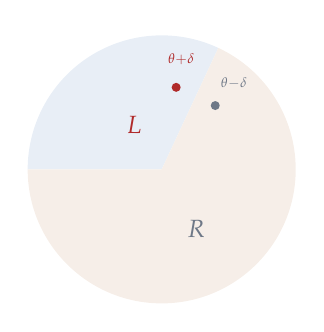
\begin{tikzpicture}[scale=0.92]
  \fill[fill1] (0,0) -- (65:1.85) arc[start angle=65,end angle=180,radius=1.85] -- cycle;
  \fill[fill2] (0,0) -- (180:1.85) arc[start angle=180,end angle=425,radius=1.85] -- cycle;
  \vertexframe{65}{south}
  \node[jcutdot] at (80:1.15) {}; \node[cut,font=\tiny] at (80:1.55) {$\theta\!+\!\delta$};
  \node[jdot,fill=aux] at (50:1.15) {}; \node[aux,font=\tiny] at (50:1.55) {$\theta\!-\!\delta$};
  \node[cut,font=\small] at (122:0.72) {$L$};
  \node[aux,font=\small] at (300:0.95) {$R$};
\end{tikzpicture}\\[2pt]
{\small (a) a left turn}\end{minipage}\hfill
\begin{minipage}{0.47\textwidth}\centering
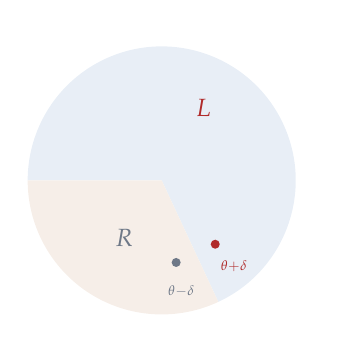
\begin{tikzpicture}[scale=0.92]
  \fill[fill1] (0,0) -- (295:1.85) arc[start angle=295,end angle=540,radius=1.85] -- cycle;
  \fill[fill2] (0,0) -- (180:1.85) arc[start angle=180,end angle=295,radius=1.85] -- cycle;
  \vertexframe{295}{north}
  \node[jcutdot] at (310:1.15) {}; \node[cut,font=\tiny] at (310:1.55) {$\theta\!+\!\delta$};
  \node[jdot,fill=aux] at (280:1.15) {}; \node[aux,font=\tiny] at (280:1.55) {$\theta\!-\!\delta$};
  \node[cut,font=\small] at (60:1.15) {$L$};
  \node[aux,font=\small] at (237:0.95) {$R$};
\end{tikzpicture}\\[2pt]
{\small (b) a right turn}\end{minipage}
\caption{The bookkeeping at a vertex. With the incoming tangent at
angle $0$, the two left germs (red) sit at polar angles $\pi-\delta$
and $\theta+\delta$, the two right germs (grey) at $\pi+\delta$ and
$\theta-\delta$. Whatever the sign of the turn, the left pair lies in
the counterclockwise arc from $\theta$ to $\pi$ --- shaded $L$ --- and
the right pair in the complementary arc. This is why the two tracks of
a strip never change places, and why they close up after a full
circuit.}\label{fig:vertex}
\end{figure}

\begin{lemma}[Two-sided strips]\label{lem:strip}
Let $P$ be a simple closed polygonal curve, or a simple polygonal arc
with a compact subarc $K$ of $P\setminus\partial P$. Then $P$
(respectively $K$) has an open neighborhood $N$, inside any prescribed
open set containing it, with
$N\setminus P=N_L\sqcup N_R$, both open and connected. Moreover, for
every $x\in P$ (resp.\ $x\in K$) and every sufficiently small disk $B$
at $x$, the set $B\setminus P$ has exactly two components, one in
$N_L$ and one in $N_R$.
\end{lemma}
\begin{proof}
Delete vertices at which consecutive edges are collinear, and orient
$P$. Around each remaining vertex take a small closed disk; around
each edge a thin rectangular block, extended slightly into its two
vertex disks. By Lemma~\ref{lem:sep}, all these can be chosen so that
only consecutive blocks overlap, and only in small rectangles around
the radial entry segments; all closures of nonadjacent blocks are
disjoint, and no block meets a nonincident edge.

Call the side of a directed edge obtained by rotating its tangent
counterclockwise through $\pi/2$ its \emph{left}. At a vertex, put the
incoming tangent at angle $0$, so the ray back along the incoming edge
has angle $\pi$, and let the outgoing tangent have angle $\theta$.
Left-side points of the incoming and outgoing strips near the vertex
have polar angles $\pi-\delta$ and $\theta+\delta$ (Figure~\ref{fig:vertex}) for small
$\delta>0$; both lie in the counterclockwise circular arc from
$\theta$ to $\pi$, hence in the same component of the circle with the
two directions $\theta,\pi$ removed, for either sign of the turn. The
right-side angles $\pi+\delta$, $\theta-\delta$ lie in the other
component. The degenerate values are impossible: $\theta=0$ is a
deleted collinear vertex, and $\theta=\pi$ would make the two incident
segments overlap, contradicting simplicity.

Take the strips narrow enough that this matching holds inside every
vertex disk, and let $N$ be the union of the open blocks. Label each
edge strip minus its core left/right, and in each vertex disk minus
its two incident rays label the sector joining the two left
half-strips left, the other right. Overlaps occur only in the labeled
half-strips, consistently by the angle computation, so every point of
$N\setminus P$ gets one label, the labeled sets are open, and each is
connected because consecutive pieces overlap in nonempty half-strips.
For a closed curve the labels close up consistently after one
circuit, by the same computation at every vertex. For an arc, run the
construction along a slightly larger compact subarc $K'$ and cut the
two extreme strips by cross-sections beyond $K$; no cap joining the
tracks is included, and the truncated $N$ still contains a
neighborhood of each point of $K$.

Finally, a small disk $B$ at $x\in P$ inside the blocks through $x$
meets $P$ in a diameter, a bent diameter, or the two edge germs at a
vertex; in each case $B\setminus P$ has two components, each connected
and hence carrying one label, and the two carry different labels by
the sector/half-strip labeling.
\end{proof}

\section{The polygonal Jordan and crosscut theorems}\label{sec:polygonal}

Let $C$ be a simple closed polygonal curve; rotate coordinates so no
edge is horizontal. For $q=(\xi,\eta)\notin C$, let $\pi_C(q)\in\{0,1\}$
be the parity of the number of edges, oriented upward, with
$a_y\le\eta<b_y$ whose crossing of the line $y=\eta$ lies strictly
right of $q$.


\begin{remark}[The count has no degenerate cases]\label{rem:parity}
$\pi_C(q)$ is a sum over \emph{edges} satisfying an inequality, not a
count of the points where a ray meets $C$, so there is nothing to
disambiguate when the ray meets the curve badly. Since $C$ has finitely
many edges, all but finitely many rotations leave none of them
horizontal; then every edge has $a_y<b_y$, so ``oriented upward'' means
something and each active edge meets the line $y=\eta$ in exactly one
point. No edge can lie \emph{along} the ray.

Vertices at height $\eta$ are handled by the half-open condition rather
than by any hypothesis on $q$. Both edges at such a vertex cross
$y=\eta$ at the vertex itself, so they pass or fail the ``strictly
right'' test together; and where the curve runs through the vertex, the
arriving edge has $b_y=\eta$ and is not counted while the departing edge
has $a_y=\eta$ and is, contributing $1$, whereas at a local minimum both
have $a_y=\eta$ and contribute $2$, and at a local maximum both have
$b_y=\eta$ and contribute $0$. Nor does ``strictly right of $q$'' ever
have to break a tie: an active edge crossing $y=\eta$ at $q$ itself
would put $q$ on $C$.

Finally --- this is used in Lemma~\ref{lem:split} --- subdividing an
edge leaves $\pi_C$ unchanged: cutting the upward edge $a\to b$ at an
interior point $c$ replaces the condition $a_y\le\eta<b_y$ by the two
conditions $a_y\le\eta<c_y$ and $c_y\le\eta<b_y$, which partition it,
and whichever piece survives crosses $y=\eta$ where the original did.

The vertex analysis in the next proof settles a different question: not
whether the count is well defined at a fixed $q$, which is the matter
here, but whether it jumps as $\eta$ \emph{varies past} a vertex height.
\end{remark}

\begin{lemma}[Crossing parity]\label{lem:parity}
$\pi_C$ is locally constant on $\mathbb R^2\setminus C$, and the two
sides of a small disk crossing one edge have opposite parity.
\end{lemma}
\begin{proof}
Away from vertex heights, the active edges and the left-right order of
their crossings vary continuously, so the count changes only when $q$
crosses an edge. At a vertex height, pass the height across each
vertex right of $q$: a through-vertex swaps one active edge for
another, a local minimum or maximum activates or retires two at once;
vertices left of $q$ never contribute. All changes are even. For the
last claim, take (Lemma~\ref{lem:sep}(c)) a disk around an interior
edge point meeting no other part of $C$; a short horizontal segment
across the edge changes the count by exactly one.
\end{proof}

\begin{theorem}[Polygonal Jordan curve theorem]\label{thm:pjct}
$\mathbb R^2\setminus C$ has exactly two regions, one bounded and one
unbounded, both with boundary $C$.
\end{theorem}
\begin{proof}
Take a strip $N_L\sqcup C\sqcup N_R$ (Lemma~\ref{lem:strip}) and
reference points $z_L,z_R$ in the two components of a small disk at an
interior edge point. For $x\notin C$, the segment from $x$ to a
nearest point $a\in C$ avoids $C$ before $a$ (a closer point would
contradict minimality), and its final portion lies in one connected
track; hence $x$ is in the component of $z_L$ or of $z_R$: at most two
components. The reference points have opposite parity
(Lemma~\ref{lem:parity}), and parity is constant on connected sets, so
there are exactly two components. The complement of a large disk is
connected, so exactly one component is unbounded. Every point of $C$
is a limit of both tracks, hence of both components, so
$C\subseteq\partial\Omega$ for each region $\Omega$; conversely
$\partial\Omega\subseteq C$ always. Since the count vanishes far to
the right, $\pi_C$ is $0$ on the unbounded region
$\Ext(C)$ and $1$ on the bounded region $\Int(C)$.
\end{proof}

Call a Jordan curve \emph{separating} if its complement has exactly two
regions --- a bounded $\Int(C)$ and an unbounded $\Ext(C)$ --- each with
boundary all of $C$. Theorem~\ref{thm:pjct} says that every polygonal
Jordan curve is separating; Theorem~\ref{thm:jct} will delete the word
``polygonal''. The next two lemmas are needed on both sides of that
divide, so they are proved from the word \emph{separating} alone, and
never used before it has been established for the curves at hand.

A \emph{crosscut} of a region $\Omega$ is a simple arc with two
distinct endpoints on $\partial\Omega$ and all other points in
$\Omega$. If $C$ is separating and $P$ is a simple arc meeting $C$
exactly in its two endpoints, then $P^\circ$ is connected and misses
$C$, so $P$ is a crosscut of exactly one of $\Int(C),\Ext(C)$.

\begin{lemma}[Absorption]\label{lem:absorb}
Let $C$ and $J$ be separating Jordan curves, $\Omega$ a region of
$\mathbb R^2\setminus C$, and $V$ a region of $\mathbb R^2\setminus J$
with $\Omega\subseteq V$. Then $C\setminus J\subseteq V$.
\end{lemma}
\begin{proof}
$C=\partial\Omega\subseteq\overline\Omega\subseteq\overline V=V\cup J$.
\end{proof}

\begin{figure}[t]
\centering
\newcommand{\bloB}{1.6+0.20*cos(3*\t)}
\begin{minipage}{0.47\textwidth}\centering
\begin{tikzpicture}[scale=0.95]
  \path[use as bounding box] (-2.5,-2.3) rectangle (2.5,2.9);
  \fill[fill1] plot[domain=20:155,smooth,variable=\t] ({\t}:{\bloB}) -- cycle;
  \fill[fill2] plot[domain=155:380,smooth,variable=\t] ({\t}:{\bloB}) -- cycle;
  \draw[jcurve] plot[domain=0:360,smooth,variable=\t] ({\t}:{\bloB});
  \coordinate (p) at (155:{1.6+0.20*cos(3*155)});
  \coordinate (q) at (20:{1.6+0.20*cos(3*20)});
  \draw[jcut] (p) -- (q);
  \node[jcutdot] at (p) {}; \node[jcutdot] at (q) {};
  \node[cut,font=\scriptsize,anchor=east] at ($(p)+(-0.08,0.02)$) {$p$};
  \node[cut,font=\scriptsize,anchor=west] at ($(q)+(0.08,0.02)$) {$q$};
  \node[cut,font=\scriptsize] at (0.80,0.95) {$P$};
  \node[font=\small] at (0.0,1.18) {$V_1$};
  \node[font=\small] at (255:0.85) {$V_2$};
  \node[font=\scriptsize,anchor=south] at (95:1.95) {$A_1$};
  \node[font=\scriptsize,anchor=north] at (265:1.85) {$A_2$};
\end{tikzpicture}\\[2pt]
{\small (a) $P$ crosses $\Omega=\Int(C)$}\end{minipage}\hfill
\begin{minipage}{0.47\textwidth}\centering
\begin{tikzpicture}[scale=0.95]
  \path[use as bounding box] (-2.5,-2.3) rectangle (2.5,2.9);
  \coordinate (p) at (160:{1.6+0.20*cos(3*160)});
  \coordinate (q) at (20:{1.6+0.20*cos(3*20)});
  \fill[fill2,even odd rule] (-2.45,-2.25) rectangle (2.45,2.85)
     plot[domain=160:380,smooth,variable=\t] ({\t}:{\bloB}) -- (0,2.6) -- cycle;
  \fill[fill1] plot[domain=20:160,smooth,variable=\t] ({\t}:{\bloB})
     -- (0,2.6) -- cycle;
  \fill[white] plot[domain=0:360,smooth,variable=\t] ({\t}:{\bloB});
  \draw[jcurve] plot[domain=0:360,smooth,variable=\t] ({\t}:{\bloB});
  \draw[jcut] (p) -- (0,2.6) -- (q);
  \node[jcutdot] at (p) {}; \node[jcutdot] at (q) {};
  \node[cut,font=\scriptsize,anchor=east] at ($(p)+(-0.08,0)$) {$p$};
  \node[cut,font=\scriptsize,anchor=west] at ($(q)+(0.08,0)$) {$q$};
  \node[cut,font=\scriptsize,anchor=south west] at (0.06,2.6) {$P$};
  \node[font=\small] at (0.0,2.02) {$V_2$};
  \node[font=\small] at (-1.75,-1.75) {$V_1$};
  \node[font=\small] at (280:0.75) {$\Omega^\dagger$};
  \node[font=\scriptsize,anchor=east] at (-0.95,1.62) {$A_2$};
  \node[font=\scriptsize,anchor=north] at (265:1.85) {$A_1$};
\end{tikzpicture}\\[2pt]
{\small (b) $P$ crosses $\Omega=\Ext(C)$}\end{minipage}
\caption{A crosscut cuts two Jordan regions out of the side it
crosses. In (a) the two cells are the interiors $\Int(J_1),\Int(J_2)$;
in (b) --- where $\Omega^\dagger=\Int(C)$ lies inside $J_1$ --- the cell
$V_1$ is the \emph{exterior} of $J_1$, and only $V_2$ is an interior.
Stating the lemma through ``the region of $\mathbb R^2\setminus J_i$
that does not contain $\Omega^\dagger$'' covers both pictures at
once. Throughout, $\overline{V_i}\cap C=A_i$.}\label{fig:crosscut}
\end{figure}

\begin{lemma}[Crosscut cells]\label{lem:cells}
Let $C$ be a separating Jordan curve and $P$ a simple arc meeting $C$
exactly in its two endpoints $p\ne q$. Let $A_1,A_2$ be the two arcs
of $C$ from $p$ to $q$, so that $J_i=A_i\cup P$ are Jordan curves, and
assume these separating as well. Let $\Omega$ be the region of
$\mathbb R^2\setminus C$ that $P$ crosses and $\Omega^\dagger$ the
other one, and let $V_i$ be the region of $\mathbb R^2\setminus J_i$
that does \emph{not} contain $\Omega^\dagger$. Then $V_1$ and $V_2$
are two distinct components of $\Omega\setminus P$, and
$\overline{V_i}\cap C=A_i$. \textup(See Figure~\ref{fig:crosscut}.\textup)
\end{lemma}
\begin{proof}
Each $J_i$ is a Jordan curve because $A_i$ and $P$ are simple arcs
meeting exactly in their two common endpoints. The region
$\Omega^\dagger$ misses $C$ and $P$, hence misses $J_i$, and being
connected it lies in one region $W_i$ of $\mathbb R^2\setminus J_i$; so
$V_i$, the other one, is well defined. Absorption applied to
$\Omega^\dagger\subseteq W_i$ gives $C\setminus J_i\subseteq W_i$,
which is disjoint from $V_i$; and $C\cap J_i=A_i$ is disjoint from
$V_i$ too. So $V_i$ is a region missing $C$ and missing
$\Omega^\dagger$, whence $V_i\subseteq\Omega$; and $V_i$ misses
$P\subseteq J_i$. Thus $V_i\subseteq\Omega\setminus P$, while
$\partial V_i=J_i\subseteq C\cup P$ misses $\Omega\setminus P$, so
$V_i$ is a component of it (Lemma~\ref{lem:clopen}). The two are
distinct because their boundaries are: $A_1=A_2$ would force
$C=A_1\cap A_2=\{p,q\}$. Finally
$\overline{V_i}\cap C=(V_i\cup J_i)\cap C=A_i$.
\end{proof}

That is everything separation alone yields; the count is completed, in
the polygonal case, by the parity function.

\begin{lemma}[Parity splits]\label{lem:split}
Let $C$ be a simple closed polygonal curve, $P$ a simple polygonal arc
meeting $C$ exactly in its two endpoints, and $J_1,J_2$ as above, with
coordinates rotated so that no edge of $C\cup P$ is horizontal. Then
\begin{equation}\label{eq:split}
\pi_C=\pi_{J_1}+\pi_{J_2}\pmod 2
\end{equation}
at every point off $C\cup P$. In particular a point of $\Int(C)$ off
$P$ lies inside exactly one of $J_1,J_2$, and a point of $\Ext(C)$ off
$P$ lies inside both or neither.
\end{lemma}
\begin{proof}
Subdivide $C$ at the endpoints of $P$ --- harmless by
Remark~\ref{rem:parity} --- and count edge by edge: the
edges of $P$ occur in both $J_i$ and cancel, while $A_1,A_2$ partition
the edges of $C$. The two consequences restate \eqref{eq:split} using
$\pi_C=1$ on $\Int(C)$ and $\pi_C=0$ on $\Ext(C)$
(Theorem~\ref{thm:pjct}).
\end{proof}

\begin{theorem}[Polygonal crosscuts]\label{thm:pcross}
In the situation of Lemma~\ref{lem:split}, $\Omega\setminus P$ has
exactly two regions, namely $V_1$ and $V_2$; and
$\mathbb R^2\setminus(C\cup P)$ has exactly three, namely
$V_1,V_2,\Omega^\dagger$, with boundaries $J_1,J_2,C$.
\end{theorem}
\begin{proof}
By Lemma~\ref{lem:cells} the $V_i$ are two distinct components of
$\Omega\setminus P$, so only exhaustion is at issue, and it is read off
Lemma~\ref{lem:split}. If $\Omega=\Int(C)$ then
$\Omega^\dagger=\Ext(C)$ lies in $\Ext(J_i)$ for both $i$ --- being
connected, unbounded, and disjoint from $J_i$ --- so $V_i=\Int(J_i)$,
and each point of $\Int(C)\setminus P$ lies inside exactly one $J_i$,
that is, in exactly one $V_i$. If instead $\Omega=\Ext(C)$, then
$\Omega^\dagger=\Int(C)$ lies inside exactly one $J_i$, say $J_1$, so
$V_1=\Ext(J_1)$ and $V_2=\Int(J_2)$; and a point of
$\Ext(C)\setminus P$ lies inside both $J_i$ --- hence in $V_2$ --- or
inside neither --- hence in $V_1$. Finally $\Omega^\dagger$ is a region
disjoint from $C\cup P$ whose boundary $C$ misses
$\mathbb R^2\setminus(C\cup P)$, so it is the third component
(Lemma~\ref{lem:clopen}).
\end{proof}

\begin{corollary}[Alternating crosscuts meet]\label{cor:alt}
If two polygonal crosscuts of the same side of $C$ have four distinct
endpoints alternating around $C$, they intersect.
\end{corollary}
\begin{proof}
The first crosscut splits its side into $V_1,V_2$, whose closures meet
$C$ in the two complementary arcs $A_1,A_2$ between its endpoints. If
the second crosscut were disjoint from the first, its connected
interior would lie in one $V_i$ and both its endpoints in
$\overline{V_i}\cap C=A_i$; but alternation puts them in the relative
interiors of different arcs.
\end{proof}

\section{\texorpdfstring{Plane graphs and $K_{3,3}$}{Plane graphs and K3,3}}\label{sec:graphs}

A finite plane graph has distinct vertex points and simple arc edges
with pairwise disjoint interiors avoiding all vertices; loops are
forbidden, parallel edges allowed. Its \emph{faces} are the components
of the complement; one is unbounded. A graph is \emph{2-connected} if
it has at least three vertices, is connected, and stays connected
after deleting any vertex. A \emph{cycle} is a connected subgraph in
which every vertex has degree two; a two-vertex cycle consists of two
parallel edges. The realization of a cycle in a plane graph is a
Jordan curve, since its edge arcs concatenate injectively.

\begin{lemma}\label{lem:graphfacts}
\textup{(a)} An edge lies on a cycle iff deleting it does not
disconnect its endpoints.
\textup{(b)} A finite tree with exactly three leaves has exactly one
vertex of degree $\ge3$, of degree exactly $3$; all other vertices are
leaves or have degree $2$.
\textup{(c)} If two finite 2-connected graphs share two vertices,
their union is 2-connected.
\textup{(d)} Subdividing edges of a 2-connected graph, or attaching a
path (an \emph{ear}) with distinct endpoints in the graph and any
number of new internal vertices, possibly none, preserves
2-connectivity.
\textup{(e)} If $H\subseteq G$ are finite 2-connected graphs, $G$ is
obtained from $H$ by adding ears.
\textup{(f)} The union of finitely many polygonal plane graphs becomes
a plane graph after subdividing at all intersections and identifying
duplicated subsegments.
\end{lemma}
\begin{proof}
(a) One direction is clear; conversely a shortest connecting walk
avoiding the edge is a simple path, which together with the edge is a
cycle (possibly a two-vertex cycle).
(b) A tree with $n$ vertices has $n-1$ edges (an endpoint of a maximal
simple path is a leaf; delete and induct), so
$\sum_v(\deg v-2)=-2$; three leaves contribute $-3$, the rest
$\ge0$, forcing one vertex with $\deg-2=1$ and no more.
(c) Deleting one vertex leaves both graphs connected and sharing a
vertex.
(d) For a subdivision of $uv$ by $w$: deleting $x\ne w$ leaves the old
connected graph with $w$ attached to $u$ or $v$; deleting $w$ removes
the edge $uv$, and a 2-connected graph has no bridge (a bridge's
deletion would leave a component with a second vertex, whose indicated
endpoint would then be a cut vertex). For an ear: deleting an old
vertex leaves the old graph connected with the pieces of the ear
attached at the ear's endpoints; deleting a new vertex leaves the old
graph intact with two attached ear pieces. An ear with no internal
vertices is a single new edge between two existing vertices, and only
the first case arises --- deleting any vertex leaves the old graph
minus that vertex, which is connected.
(e) Given the part $H_0$ built so far, a component $L$ of $G-V(H_0)$ has
two distinct neighbors in $K$ (a unique neighbor would be a cut
vertex, since $H_0$ has other vertices and all $L$-to-$H_0$ paths pass
through it); a shortest path through $L$ between two neighbors is an
ear. When all vertices are present, add missing edges as ears.
(f) Segments intersect in nothing, a point, or an interval; subdivide
at all such points and interval endpoints.
\end{proof}

\begin{lemma}[Polygonal redrawing]\label{lem:redraw}
Every finite plane graph is isomorphic to one with polygonal edges.
\end{lemma}
\begin{proof}
Take small disjoint closed squares $D_v$ around the vertices, meeting
no nonincident edge. For an edge from $v$ to $w$, let $c_{v,e}$ be its
last point in $D_v$ and $c_{w,e}$ the first subsequent point in
$D_w$; both lie on the square boundaries, and the \emph{core} between
them avoids all square interiors and all other squares. Distinct cores
are disjoint compacta, with distinct boundary marks $c_{v,e}$. In
$M=\mathbb R^2\setminus\bigcup_vD_v^\circ$, which is locally
polygonally connected (disks, half-disks along sides, three-quarter
disks at corners), Lemma~\ref{lem:sep} yields pairwise disjoint
connected relatively open neighborhoods $U_e\supseteq K_e$ meeting the
square boundaries only in small disjoint arcs around the marks: the
boundary minus such an arc is compact and disjoint from $K_e$. The
clopen argument of Lemma~\ref{lem:polyconn} runs inside each $U_e$, so
$c_{v,e}$ and $c_{w,e}$ are joined in $U_e$ by a simple polygonal
replacement core. Finally join $v$ radially to each $c_{v,e}$ inside
the convex square; radial segments meet the square boundary only at
their marks, hence meet replacement cores only there, and distinct
radials meet only at $v$. The assembled polygonal arcs realize the
same abstract graph.
\end{proof}

\begin{figure}[t]
\centering
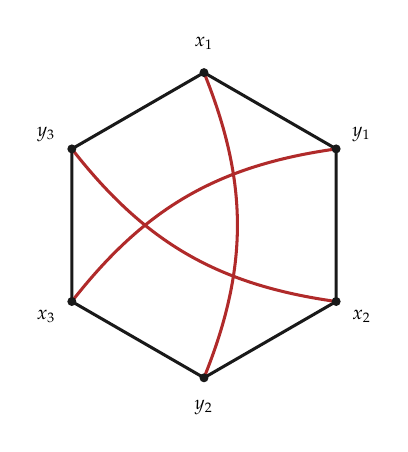
\begin{tikzpicture}[scale=1.25]
  \foreach \a/\n/\lab in {90/x1/{$x_1$},30/y1/{$y_1$},-30/x2/{$x_2$},
                          -90/y2/{$y_2$},-150/x3/{$x_3$},150/y3/{$y_3$}}
    {\coordinate (\n) at (\a:1.55); \node[font=\scriptsize] at (\a:1.85) {\lab};}
  \draw[jcurve] (x1)--(y1)--(x2)--(y2)--(x3)--(y3)--cycle;
  \draw[jcut] (x1) to[bend left=22] (y2);
  \draw[jcut] (x2) to[bend left=22] (y3);
  \draw[jcut] (x3) to[bend left=22] (y1);
  \foreach \n in {x1,y1,x2,y2,x3,y3} {\node[jdot] at (\n) {};}
\end{tikzpicture}
\caption{$K_{3,3}$ as a hexagon with three chords. Read around the
hexagon, the chords join positions $(1,4)$, $(3,6)$ and $(5,2)$, so
\emph{any two of them alternate}. In a plane drawing two of the three
would have to lie on the same side of the hexagon, where
Corollary~\ref{cor:alt} forces them to
meet.}\label{fig:k33}
\end{figure}

\begin{lemma}\label{lem:k33}
No subdivision of $K_{3,3}$ has a plane drawing.
\end{lemma}
\begin{proof}
In a drawing of a subdivision, each branch path is a simple arc and
distinct branch paths share at most branch vertices, so a drawing of
$K_{3,3}$ itself results; make it polygonal
(Lemma~\ref{lem:redraw}). View $K_{3,3}$ as the hexagon
$x_1y_1x_2y_2x_3y_3$ plus the chords $x_1y_2,x_2y_3,x_3y_1$
(Figure~\ref{fig:k33}). Each
chord lies on one side of the hexagon; two lie on the same side; and
each pair of chords has alternating endpoints (positions
$(1,4),(3,6),(5,2)$ pairwise alternate), contradicting
Corollary~\ref{cor:alt}.
\end{proof}

\begin{lemma}[Face cycles]\label{lem:facecycles}
Every face of a finite 2-connected polygonal plane graph is one of the
two regions of a cycle of the graph, its boundary cycle; bounded faces
are interiors of their boundary cycles.
\end{lemma}
\begin{proof}
Every vertex has two distinct neighbors (a sole neighbor would be a
cut vertex), so an endpoint of a maximal simple path closes a cycle of
length $\ge3$. Build the graph from that cycle by ears
(Lemma~\ref{lem:graphfacts}(e)) and induct: an ear's interior is
connected and disjoint from the current graph, so it lies in one
current face $F$, one side of its boundary cycle; the ear's endpoints,
limits of its interior, lie on $\partial F$; so the ear is a crosscut,
and Theorem~\ref{thm:pcross} replaces $F$ by two regions bounded by
cycles (possibly two-vertex cycles), leaving other faces untouched.
\end{proof}

\begin{lemma}[Outer face of a chain]\label{lem:chain}
Let $\Gamma_1,\dots,\Gamma_k$ \textup($k\ge3$\textup) be finite
2-connected polygonal plane graphs, consecutive ones sharing at least
two vertices \textup(after subdividing common points\textup),
nonconsecutive ones disjoint. A point lying in the outer face of every
consecutive union $\Gamma_i\cup\Gamma_{i+1}$ lies in the outer face of
the whole union $G$.
\end{lemma}
\begin{proof}
$G$ is 2-connected by Lemma~\ref{lem:graphfacts}(c). If $x$ lay in a
bounded face, some cycle of $G$ would enclose it
(Lemma~\ref{lem:facecycles}). Choose $i\le j$ with $j-i$ minimal so
that a cycle in $\Gamma_i\cup\cdots\cup\Gamma_j$ encloses $x$. If
$j-i\le1$, a consecutive pair $H$ contains that union; the face of $H$
containing $x$ is connected, disjoint from the cycle, and meets its
interior, hence lies inside it and is bounded --- contradicting the
hypothesis. So $j-i\ge2$; among enclosing cycles in this fixed union
pick $C$ with fewest edges outside $\Gamma_{j-1}$. Interval minimality
forces on $C$ an edge of $\Gamma_j$ outside $\Gamma_{j-1}$ and an
earlier-chain edge outside $\Gamma_{j-1}$ (else shrink the interval;
note $\Gamma_j$ is disjoint from all $\Gamma_\ell$, $\ell\le j-2$).
Pick interior points $a,b$ of those two edges; each of the two arcs of
$C$ from $a$ to $b$ must meet $\Gamma_{j-1}$, since consecutive
$C$-edges of the two outside types cannot share a vertex. Hence
$C\cap\Gamma_{j-1}$ has at least two maximal subpaths, one per arc,
and distinct maximal subpaths are vertex-disjoint. Let $R$ be a
shortest path in the connected graph $\Gamma_{j-1}$ from one such
subpath $P$ to $V(C)\setminus V(P)$: its internal vertices avoid $C$
(a $C$-vertex inside $R$ would shorten it), its endpoints $u,v$ lie on
different maximal subpaths, and its edges are not $C$-edges (a single
$C$-edge from $u$ would stay inside $P$ by maximality). Then $R$ is a
geometric crosscut of one side of $C$; each of the two arcs
$C_1,C_2$ of $C$ between $u,v$ contains an edge outside
$\Gamma_{j-1}$, since its ends lie on different maximal subpaths. Since
$x$ lies inside $C$ and off $R$, Lemma~\ref{lem:split} says that
exactly one of the cycles $R\cup C_1$,
$R\cup C_2$ encloses $x$; it lies in the same union and has strictly
fewer edges outside $\Gamma_{j-1}$, a contradiction. So no bounded
face contains $x$.
\end{proof}

\section{Arc complements and the Jordan curve theorem}\label{sec:jct}

Two statements separate the polygonal theory from the general one: an arc
separates nothing, and a curve separates into exactly two. The first is
proved by burying the arc in a chain of small squares and appealing to
Lemma~\ref{lem:chain}; the second, in both directions, by exhibiting a
plane $K_{3,3}$.

\begin{figure}[t]
\centering
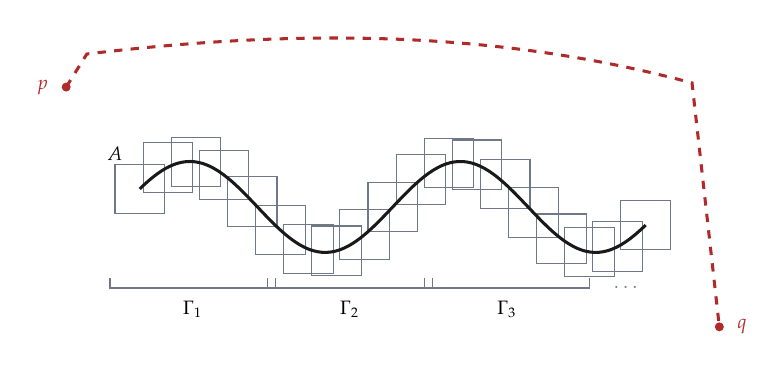
\begin{tikzpicture}[scale=1.05]
  \foreach \i in {0,...,18} {
    \pgfmathsetmacro{\tx}{-3.06+0.34*\i}
    \pgfmathsetmacro{\ty}{0.55*sin(110*\tx)}
    \draw[aux,line width=0.4pt] (\tx-0.30,\ty-0.30) rectangle (\tx+0.30,\ty+0.30);}
  \draw[jcurve,domain=-3.06:3.06,smooth,variable=\x,samples=120]
    plot (\x,{0.55*sin(110*\x)});
  \draw[jcut,dashed] (-3.95,1.45) -- (-3.7,1.85)
     .. controls (-1.2,2.15) and (1.2,2.15) .. (3.62,1.5) -- (3.95,-1.45);
  \node[jcutdot] at (-3.95,1.45) {}; \node[jcutdot] at (3.95,-1.45) {};
  \node[cut,font=\scriptsize,anchor=east] at (-4.05,1.45) {$p$};
  \node[cut,font=\scriptsize,anchor=west] at (4.05,-1.45) {$q$};
  \node[font=\scriptsize,anchor=north east] at (-3.15,0.85) {$A$};
  \foreach \l/\r/\lab in {-3.42/-1.42/{$\Gamma_1$},-1.52/0.48/{$\Gamma_2$},
                          0.38/2.38/{$\Gamma_3$}} {
    \draw[aux,line width=0.4pt] (\l,-0.86) -- (\l,-0.98) -- (\r,-0.98) -- (\r,-0.86);
    \node[font=\scriptsize,anchor=north] at ({(\l+\r)/2},-1.02) {\lab};}
  \node[aux,font=\scriptsize,anchor=west] at (2.55,-0.98) {$\cdots$};
\end{tikzpicture}
\caption{Why an arc cannot separate. Small squares of radius $\delta/4$
are strung along $A$ so that consecutive ones overlap; blocks of them
form 2-connected graphs $\Gamma_i$, consecutive blocks sharing a whole
square and non-consecutive ones disjoint. The chain lemma says the outer
face of the union is a single region --- a corridor running all the way
around --- and it contains both $p$ and $q$. The arc itself is buried:
each of its points lies inside or on one of the
squares.}\label{fig:chain}
\end{figure}

\begin{theorem}[Arc-complement theorem]\label{thm:arc}
The complement of a simple arc $A$ is connected.
\end{theorem}
\begin{proof}
Given $p,q\notin A$, choose $d>0$ so that both points are at
$\ell^\infty$-distance $>4d$ from $A$. By uniform continuity split $A=A_1\cup\cdots\cup A_k$ ($k\ge3$) into
subarcs of $\ell^\infty$-diameter $<d$ from their initial points
$a_i$, and let $d'>0$ be the least $\ell^\infty$-distance between
nonadjacent subarcs (Lemma~\ref{lem:sep}(b)); put
$\delta=\min(d,d')$. Every distance in this proof is $\ell^\infty$, to
match the squares about to be drawn. Sample each
$A_i$ so finely that every point of the subarc between two consecutive
samples is within $\delta/4$ of the earlier one (hence in particular
consecutive samples are within $\delta/4$), taking the common endpoint
of adjacent subarcs as a sample for both, and
around every sample draw the boundary of the $\ell^\infty$-square of
radius $\delta/4$; let $\Gamma_i$ be the overlay of the $A_i$-squares.
Two consecutive squares coincide, or are distinct congruent squares
with centers $c\ne c'$ at distance $m=\|c-c'\|_\infty\le\delta/4$. In
the second case their boundaries meet in at least two points. They meet
at all: travelling from $c$ toward $c'$ until the first boundary is
reached lands at $z=c+(\delta/4)(c'-c)/m$, and
$\|z-c'\|_\infty=\delta/4-m<\delta/4$, so $z$ is interior to the second
square, while the first boundary is not contained in the second square
--- a square is the convex hull of its boundary, so that would put the
whole first square inside the second, and congruent squares one inside
the other coincide. So the first boundary meets both the interior and
the complement of the second square; were the two boundaries to share
exactly one point, that circle minus a point --- still connected ---
would split into two nonempty relatively open pieces. Hence each
$\Gamma_i$ is 2-connected by Lemma~\ref{lem:graphfacts}(c,d), and
consecutive $\Gamma_i$ share a whole square, while for $|i-j|\ge2$ the
graphs are disjoint ($\delta$ apart minus radii $\delta/2$). Each pair
$\Gamma_i\cup\Gamma_{i+1}$ lies in the square of radius $3d$ about
$a_i$ (its centers are within $d$ or within $2d$ of $a_i$, and the
square radius is $\delta/4\le d/4$), so $p,q$ lie in the outer
face of every pair (Figure~\ref{fig:chain}), hence of $G=\bigcup\Gamma_i$
(Lemma~\ref{lem:chain}). Every point of $A$ lies in or on a small
square; interior points are separated from the outer face by the
square's boundary cycle, boundary points lie on $G$. So the outer
face, a region, avoids $A$ and joins $p$ to $q$
(Lemma~\ref{lem:polyconn}).
\end{proof}

\begin{lemma}[Circular parametrization]\label{lem:circle}
A Jordan curve $C$ is homeomorphic to the unit circle (and to the
boundary of a square); any two of its points split it into two arcs
meeting only there, and its open subarcs are a basis of its topology.
\end{lemma}
\begin{proof}
Let $e(t)=(\cos2\pi t,\sin2\pi t)$ and set $h(e(t))=\gamma(t)$: well
defined and bijective. If $z_n\to z$, lifts $t_n$ have, along any
subsequence, a further subsequence converging to some $t$ with
$e(t)=z$, along which $h(z_n)\to h(z)$; hence $h$ is continuous, and
being a continuous bijection from a compactum to a Hausdorff space, a
homeomorphism. The remaining claims transport from the circle; the
square case follows via radial projection.
\end{proof}

\begin{figure}[t]
\centering
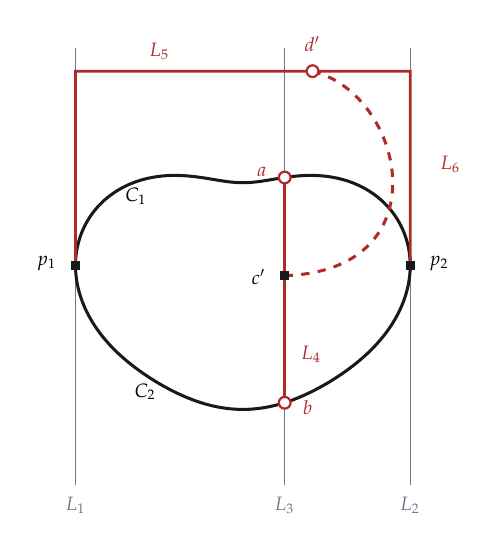
\begin{tikzpicture}[scale=1.18]
  \def\blb{1.5+0.28*cos(2*\t)+0.12*sin(3*\t)}
  \coordinate (p1) at (-1.801,0.209);
  \coordinate (p2) at (1.801,0.209);
  \coordinate (a)  at (0.45,1.156);
  \coordinate (b)  at (0.45,-1.268);
  \coordinate (cp) at (0.45,0.10);
  \coordinate (dp) at (0.75,2.30);
  \draw[aux,line width=0.4pt] (-1.801,-2.15) -- (-1.801,2.55);
  \draw[aux,line width=0.4pt] (1.801,-2.15) -- (1.801,2.55);
  \draw[aux,line width=0.4pt] (0.45,-2.15) -- (0.45,2.55);
  \node[aux,font=\scriptsize,anchor=north] at (-1.801,-2.18) {$L_1$};
  \node[aux,font=\scriptsize,anchor=north] at (1.801,-2.18) {$L_2$};
  \node[aux,font=\scriptsize,anchor=north] at (0.45,-2.18) {$L_3$};
  \draw[jcurve,domain=0:360,smooth,variable=\t,samples=200]
    plot ({\t}:{\blb});
  \draw[cut,line width=1.0pt] (a) -- (b);
  \draw[cut,line width=1.0pt] (p1) -- (-1.801,2.30) -- (1.801,2.30) -- (p2);
  \draw[jcut,dashed] (cp) .. controls (2.15,0.15) and (1.75,2.05) .. (dp);
  \foreach \n in {p1,p2,cp} {\node[rectangle,fill=curve,inner sep=1.7pt] at (\n) {};}
  \foreach \n in {a,b,dp} {\node[circle,draw=cut,fill=white,line width=0.8pt,
      inner sep=1.5pt] at (\n) {};}
  \node[font=\scriptsize,anchor=east]  at ($(p1)+(-0.10,0.02)$) {$p_1$};
  \node[font=\scriptsize,anchor=west]  at ($(p2)+(0.10,0.02)$) {$p_2$};
  \node[cut,font=\scriptsize,anchor=east] at ($(a)+(-0.09,0.06)$) {$a$};
  \node[cut,font=\scriptsize,anchor=west] at ($(b)+(0.09,-0.05)$) {$b$};
  \node[font=\scriptsize,anchor=east]  at ($(cp)+(-0.10,-0.02)$) {$c'$};
  \node[cut,font=\scriptsize,anchor=south] at ($(dp)+(0,0.10)$) {$d'$};
  \node[cut,font=\scriptsize,anchor=west] at (0.52,-0.75) {$L_4$};
  \node[cut,font=\scriptsize,anchor=south] at (-0.9,2.32) {$L_5$};
  \node[cut,font=\scriptsize,anchor=west] at (2.02,1.30) {$L_6$};
  \node[font=\scriptsize] at (-1.15,0.95) {$C_1$};
  \node[font=\scriptsize] at (-1.05,-1.15) {$C_2$};
\end{tikzpicture}
\caption{The configuration behind ``a Jordan curve separates''. Squares
mark $p_1,p_2,c'$; circles mark $a,b,d'$. Every square is joined to
every circle by one of nine internally disjoint arcs --- four subarcs of
$C$, two halves of $L_4$, two pieces of $L_5$, and $L_6$ --- so the
picture is a plane subdivision of $K_{3,3}$, which cannot exist. The
dashed $L_6$ is the hypothesis being refuted --- it is assumed to reach
$L_5$ from $L_4$ without meeting $C$ --- so no drawing of it can be
faithful; here it is shown crossing $C$ on the
right.}\label{fig:sep}
\end{figure}

\begin{proposition}[A Jordan curve separates]\label{prop:sep}
$\mathbb R^2\setminus C$ is disconnected.
\end{proposition}
\begin{proof}
$C$ is not contained in a line: it would be a nondegenerate compact
connected subset of it, a closed interval, which one interior point
disconnects, while the circle minus a point is connected. Rotate so
the horizontal width is positive; let $L_1,L_2$ be the vertical
supporting lines, $p_i$ the highest point of $C\cap L_i$, and
$C_1,C_2$ the two arcs of $C$ between $p_1,p_2$. A vertical line
$L_3$ strictly between meets both arcs (their horizontal projections
are connected and contain both extremes). The compact sets
$C_i\cap L_3$ are disjoint (the $p_i$ are off $L_3$); choose a closest
pair $a\in C_1$, $b\in C_2$ on $L_3$; the open segment between them
misses $C$, since a $C$-point on it, lying on some $C_i$, would be
closer to the other endpoint. Call the closed segment $L_4$. Join
$p_1$ to $p_2$ by the polygonal path $L_5$ running up the supporting
lines and across a horizontal line above $C$; each interior point of
$L_5$ reaches infinity by a horizontal ray away from the strip or a
vertical ray upward, missing $C$, so the interior of $L_5$ lies in the
unbounded component; and $L_4\cap L_5=\varnothing$.

Suppose $L_4\setminus\{a,b\}$ also lay in the unbounded component.
Join an interior point $c$ of $L_4$ to an interior point $d$ of $L_5$
by a simple polygonal arc $R$ in that component
(Lemma~\ref{lem:polyconn}); let $c'$ be the last point of $R$ on
$L_4$ and $d'$ its first subsequent point on $L_5$, and $L_6$ the
subarc between, meeting $L_4\cup L_5$ only at its ends and missing
$C$. Then $C\cup L_4\cup L_5\cup L_6$ is a plane subdivision of
$K_{3,3}$ with parts $\{p_1,p_2,c'\}$ and $\{a,b,d'\}$
(Figure~\ref{fig:sep}): the four
subarcs of $C_1,C_2$ cut at $a,b$, the two subsegments of $L_4$ cut at
$c'$, the two subpaths of $L_5$ cut at $d'$, and $L_6$ are nine
internally disjoint branch paths (all the required disjointness is by
construction: $C$ meets $L_4$ in $\{a,b\}$, $L_5$ in $\{p_1,p_2\}$,
$L_6$ not at all, and the six branch vertices are distinct since
$c',d'$ are off $C$). This contradicts Lemma~\ref{lem:k33}; so some
point of $L_4$ lies outside the unbounded component, and the
complement is disconnected.
\end{proof}

\begin{lemma}[Accessible points are dense]\label{lem:accdense}
Let $\Omega$ be a component of $\mathbb R^2\setminus C$ and
$x\in\Omega$. The points of $C$ reachable from $x$ by a polygonal arc
meeting $C$ only at its endpoint are dense in $C$.
\end{lemma}
\begin{proof}
Take $y$ in another component and an open arc $J_0$ with closure
inside the given open arc $J$ of $C$. Then $C\setminus J_0$ is a
simple arc, so its complement is connected (Theorem~\ref{thm:arc});
join $x$ to $y$ there by a simple polygonal arc. The arc must cross
$C$, and only inside $J_0$; its first meeting, from $x$, is the
endpoint of an access arc from $\Omega$ and lies in $J$.
\end{proof}

\begin{figure}[t]
\centering
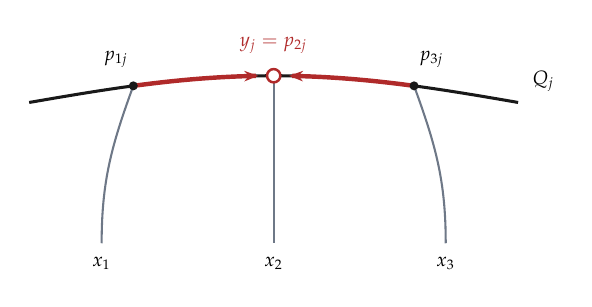
\begin{tikzpicture}[scale=1.15]
  \draw[jcurve,domain=-2.7:2.7,smooth,variable=\x,samples=80]
     plot (\x,{0.30*cos(33*\x)});
  \coordinate (t1) at (-1.55,{0.30*cos(33*(-1.55))});
  \coordinate (t2) at (0,0.30);
  \coordinate (t3) at (1.55,{0.30*cos(33*1.55)});
  \draw[cut,line width=1.6pt,-{Stealth[length=5pt]},
        domain=-1.55:-0.17,smooth,variable=\x,samples=40]
     plot (\x,{0.30*cos(33*\x)});
  \draw[cut,line width=1.6pt,{Stealth[length=5pt]}-,
        domain=0.17:1.55,smooth,variable=\x,samples=40]
     plot (\x,{0.30*cos(33*\x)});
  \draw[aux,line width=0.75pt] (t1) to[out=-110,in=90] (-1.9,-1.55);
  \draw[aux,line width=0.75pt] (t2) to[out=-90,in=90] (0,-1.55);
  \draw[aux,line width=0.75pt] (t3) to[out=-70,in=90] (1.9,-1.55);
  \node[font=\scriptsize,anchor=north] at (-1.9,-1.6) {$x_1$};
  \node[font=\scriptsize,anchor=north] at (0,-1.6) {$x_2$};
  \node[font=\scriptsize,anchor=north] at (1.9,-1.6) {$x_3$};
  \foreach \n in {t1,t3} {\node[jdot] at (\n) {};}
  \node[circle,draw=cut,fill=white,line width=0.9pt,inner sep=1.7pt] at (t2) {};
  \node[font=\scriptsize,anchor=south east] at ($(t1)+(0.05,0.10)$) {$p_{1j}$};
  \node[font=\scriptsize,anchor=south west] at ($(t3)+(-0.05,0.10)$) {$p_{3j}$};
  \node[cut,font=\scriptsize,anchor=south] at ($(t2)+(0,0.14)$) {$y_j=p_{2j}$};
  \node[font=\scriptsize,anchor=west] at (2.75,0.24) {$Q_j$};
\end{tikzpicture}
\caption{The middle-terminal trick. On the arc $Q_j$ the three trees
land at $p_{1j},p_{2j},p_{3j}$; the meeting point $y_j$ is chosen to be
the \emph{middle} one. The two travelling subarcs (thick) then reach
$y_j$ from opposite sides and share no interior point, while the tree
that lands on $y_j$ travels not at all. Choosing any other terminal as
$y_j$ would make two of the three routes overlap.}\label{fig:middle}
\end{figure}

\begin{theorem}[Jordan curve theorem]\label{thm:jct}
$\mathbb R^2\setminus C$ has exactly two regions, one bounded and one
unbounded, both with boundary $C$.
\end{theorem}
\begin{proof}
At least two components exist (Proposition~\ref{prop:sep}). Suppose
$\Omega_1,\Omega_2,\Omega_3$ were three. Split $C$ into three closed
arcs $Q_1,Q_2,Q_3$ with disjoint relative interiors, pick
$q_i\in\Omega_i$, and choose nine distinct points $p_{ij}$ in the
relative interiors of the $Q_j$, each accessible from $q_i$
(Lemma~\ref{lem:accdense}; a dense set meets every open subarc even
after finitely many deletions, since otherwise a nonempty open subarc
would avoid it). Overlay the three access arcs from $q_i$ and take a
minimal connected subgraph $T_i$ spanning $p_{i1},p_{i2},p_{i3}$: a
tree (a cycle edge could be deleted) in which each terminal has degree
one, because other access arcs of $q_i$ meet $C$ only at their own
distinct endpoints; minimality forbids other leaves. By
Lemma~\ref{lem:graphfacts}(b), $T_i$ is three internally disjoint
branches from a center $x_i$ to the terminals. The $T_i$ are pairwise
disjoint: their interiors lie in distinct components and the nine
terminals are distinct. On each $Q_j$ let $y_j$ be the middle of the
three terminals (Figure~\ref{fig:middle}), and join each $x_i$ to each $y_j$ by its branch to
$p_{ij}$ followed by the subarc of $Q_j$ to $y_j$ (empty for the
middle terminal). These nine paths are internally disjoint: branches
within one tree are; trees are disjoint; the two nonempty $Q_j$-subarcs
approach $y_j$ from opposite sides; and subarcs lie in the disjoint
relative interiors of the $Q_j$, which the branches meet only at their
own terminals. This is a plane subdivision of $K_{3,3}$ with parts
$\{x_i\}$, $\{y_j\}$, contradicting Lemma~\ref{lem:k33}. So there are
exactly two components; accessibility from both makes every point of
$C$ a boundary point of both, boundaries lie in $C$, and exactly one
component is unbounded.
\end{proof}

Every Jordan curve is therefore separating, and the two lemmas of
Section~\ref{sec:polygonal} that were proved from that word alone ---
absorption and crosscut cells --- are from now on available for all of
them.

\section{Crosscuts of Jordan domains; reduction to the square}\label{sec:reduce}

From here $C$ is an arbitrary Jordan curve and $D=\Int(C)$. The crosscut
theorem below is the instrument Part~II uses at every single step; after
it, the main theorem is reduced to the case of a square, and the rest of
the paper is the construction that handles that case.

\begin{lemma}[At most two sides]\label{lem:twosides}
If $P$ is a polygonal crosscut of $D=\Int(C)$, then $D\setminus P$ has
at most two components.
\end{lemma}
\begin{proof}
Fix $z_0$ interior to a straight edge of $P$ and, by
Lemma~\ref{lem:sep}(c), a closed disk $B\subseteq D$ meeting $P$ in a
straight diameter; let $z_L,z_R$ be points of its two half-disks.
Given $x\in D\setminus P$, join $x$ to $z_0$ by a polygonal arc
$\gamma$ in the region $D$ and let $z$ be its first point on $P$
(interior to $P$, since the endpoints of $P$ are on $C$). If $z=z_0$,
the part of $\gamma$ just before $z_0$ lies in one half-disk, joined
to $z_L$ or $z_R$ inside $B\setminus P$. Otherwise take the compact
subarc $K$ of $P$ from $z$ to $z_0$ and a strip $N\subseteq D$ around
$K$ with $N\setminus P=N_L\sqcup N_R$ (Lemma~\ref{lem:strip}); note
the strip removes all of $P$, not only $K$. The point of $\gamma$ just
before $z$ lies in one track; a small disk at $z_0$ has its two
components inside the two tracks, so that track reaches one half-disk
of $B$. In all cases $x$ is joined in $D\setminus P$ to $z_L$ or
$z_R$, so there are at most two components.
\end{proof}

\begin{theorem}[Crosscut theorem]\label{thm:cross}
A polygonal crosscut $P$ of $D=\Int(C)$ with endpoints $p,q$ splits
$D$ into exactly two regions, namely $\Int(A_1\cup P)$ and
$\Int(A_2\cup P)$, where $A_1,A_2$ are the two arcs of $C$ from $p$ to
$q$; and $\mathbb R^2\setminus(C\cup P)$ has exactly three regions,
with boundaries $C$, $A_1\cup P$, $A_2\cup P$.
\end{theorem}
\begin{proof}
Each $J_i=A_i\cup P$ is a Jordan curve, and all three of $C,J_1,J_2$
are separating by Theorem~\ref{thm:jct}; so Lemma~\ref{lem:cells}
applies with $\Omega=D$. Here $\Omega^\dagger=\Ext(C)$ is connected,
unbounded and disjoint from $J_i$, hence lies in $\Ext(J_i)$, so the
lemma's $V_i$ is $\Int(J_i)$: the two regions $\Int(J_1),\Int(J_2)$ are
distinct components of $D\setminus P$, and by
Lemma~\ref{lem:twosides} they are the only ones. Finally $\Ext(C)$ is
a region disjoint from $C\cup P$ whose boundary $C$ misses
$\mathbb R^2\setminus(C\cup P)$, so it is the third component
(Lemma~\ref{lem:clopen}); the boundaries are those given by
Theorem~\ref{thm:jct} for $C,J_1,J_2$.
\end{proof}

\begin{lemma}[Accessible endpoints can be joined]\label{lem:join}
Let $F$ be a region and
let $a\ne b$ be points of $\partial F$ each accessible from $F$ by a
polygonal arc meeting $\partial F$ only at its endpoint. Then there is
a polygonal crosscut of $F$ from $a$ to $b$.
\end{lemma}
\begin{proof}
Join the inner endpoints of the two access arcs by a polygonal arc in
the region $F$ (Lemma~\ref{lem:polyconn}). The union meets
$\partial F$ only in $\{a,b\}$, and $a,b$ have degree one in its
subdivision graph; extract the simple polygonal path from $a$ to $b$
(Lemma~\ref{lem:polyconn}).
\end{proof}

\begin{theorem}[Square extension]\label{thm:square}
With $Q=[-1,1]^2$ and $S=\partial Q$: every homeomorphism $u:C\to S$
extends to a homeomorphism $\overline F:C\cup\Int(C)\to Q$.
\end{theorem}

\begin{proposition}[Reduction to the square]\label{prop:reduce}
Theorem~\ref{thm:square} implies that every homeomorphism $f:C\to C'$
extends to a homeomorphism
$C\cup\Int(C)\to C'\cup\Int(C')$.
\end{proposition}
\begin{proof}
Choose $h:C'\to S$ (Lemma~\ref{lem:circle}), extend $h\circ f$ and $h$
to $\Phi,\Psi$ by Theorem~\ref{thm:square}, and take
$\Psi^{-1}\circ\Phi$.
\end{proof}

The next five sections prove Theorem~\ref{thm:square}. Fix $C$, $u$,
and write
$D=\Int(C)$, $\overline D=C\cup D$.

\emph{Strong accessibility.} A point $p\in C$ is \emph{strongly
accessible} if some open disk $B(q,r)\subseteq D$ has $\|q-p\|=r$. If
$q\in D$ and $a$ is a nearest point of $C$, then $B(q,\|q-a\|)$ misses
$C$ and, being connected, lies in $D$: nearest points are strongly
accessible. If $B(q,r)$ witnesses $p$ and $v=(q-p)/r$, then for every
unit $w$ with $\langle v,w\rangle>\tfrac12$ and $0<t<r$,
\[
\|p+tw-q\|^2=r^2+t^2-2\,t\,r\,\langle v,w\rangle<r^2+t(t-r)<r^2,
\]
so a whole open cone of short straight segments at $p$ enters
$B(q,r)\subseteq D$. Taking a nearest point $a(q)\in C$ for every
$q\in\mathbb Q^2\cap D$ gives a countable set $\mathcal A$ of strongly
accessible points, dense in $C$ because $C=\partial D$
(Theorem~\ref{thm:jct}) gives rational $q$ with $\|q-p\|<\varepsilon/2$
and then $\|a(q)-p\|\le2\|q-p\|<\varepsilon$. Fix this $\mathcal A$.

\section{Matched cellulations}\label{sec:cell}

\begin{proposition}[Initial pair]\label{prop:init}
Subdivide $C$ at six boundary vertices: the four $u$-preimages of the
corners of $Q$, and two further points $a,b\in\mathcal A$ chosen in two
nonadjacent corner arcs, so that $u(a),u(b)$ lie in the relative
interiors of opposite sides of $Q$; subdivide $S$ correspondingly.
There is a polygonal crosscut $P$ of $D$ from $a$ to $b$, and the
straight chord $P'=[u(a),u(b)]$ is a crosscut of $Q^\circ$. The
crosscut theorem splits $\overline D$ and $Q$ into two closed cells
each, and the sides correspond by
$\overline{R_i}\cap C=A_i\leftrightarrow
\overline{R_i'}\cap S=u(A_i)$, where $A_1,A_2$ are the two arcs of
$C$ from $a$ to $b$, each realized as a path of boundary edges.
\end{proposition}
\begin{proof}
The dense set $\mathcal A$ meets both chosen open corner arcs, even after any
finite exclusions. Short straight access segments at $a,b$ exist by
strong accessibility, and Lemma~\ref{lem:join} gives $P$. Since
$u(a),u(b)$ are interior to opposite sides, the interior of
$[u(a),u(b)]$ lies in $Q^\circ$ by convexity. Apply
Theorem~\ref{thm:cross} on both sides (for the square, its polygonal
case). Each skeleton --- a six-vertex cycle plus a chord --- is
2-connected, and its open inner part, the open chord, is
connected.
\end{proof}

A \emph{cellulation} of $\overline D$ is a finite partition of
$\overline D$ into open \emph{cells} --- points (\emph{vertices}), open
arcs (\emph{edges}), and regions (\emph{faces}) --- obtained from the
decomposition of Proposition~\ref{prop:init} by finitely many
applications of the two constructors below; a cellulation of $Q$ is the
same with $S$ in place of $C$. The initial cellulation consists of the
six boundary vertices, the six outer edges, the crosscut, and the two
faces. The constructors are:
\begin{itemize}
\item[(i)] \emph{edge subdivision}: choose an interior point of an edge
$e$ and replace $e$ by that point and the two edges it cuts $e$ into;
\item[(ii)] \emph{face split}: choose a face $R$ and two distinct
vertices on its boundary, insert a crosscut of $R$ joining them, and
replace $R$ by the crosscut's interior and the two regions the crosscut
cuts off.
\end{itemize}
Cells contained in $C$ (resp.\ $S$) are \emph{outer}, the rest
\emph{inner}; inner edges are always polygonal arcs with interiors in
$D$ (resp.\ $Q^\circ$). The \emph{carrier} of a point is the cell
containing it. Write $\sigma\preceq\tau$ (``$\sigma$ is a subcell of
$\tau$'') when $\sigma\subseteq\overline\tau$, and let the
\emph{closed star} $\St(\sigma)$ be the union of the closures of the
supercells of $\sigma$.

A \emph{matched pair} is a cellulation of $\overline D$ together with
one of $Q$ built by the \emph{same} sequence of constructors, and a
homeomorphism $g$ of the two $1$-skeletons which restricts to $u$ on
$C$ and carries every vertex and edge to its counterpart. To apply a
constructor to a matched pair is to apply it on both sides at once: a
subdivision inserts corresponding points (via $g$, hence via $u$ on
outer edges); a split inserts crosscuts of corresponding faces between
corresponding vertices, $g$ is extended over them by any homeomorphism
fixing the endpoints, and the two new faces on each side are matched by
their boundary paths, which correspond.

Three lemmas record what this arrangement provides. The first is
geometry and holds in either realization separately; the second is
bookkeeping; the third is the reason for the whole construction.

\begin{lemma}[Cell geometry]\label{lem:cellgeom}
In any cellulation:
\textup{(a)} the open cells partition the closed domain, and every
closed cell is the disjoint union of the open cells it contains;
\textup{(b)} \textup(frontier\textup) an open cell that meets the
closure of a cell is contained in it;
\textup{(c)} every face is the interior of a Jordan curve assembled
from closed cells, its \emph{boundary cycle}; every boundary cycle
contains an inner edge; every outer edge lies on exactly one boundary
cycle;
\textup{(d)} distinct faces are incomparable under $\preceq$.
\end{lemma}
\begin{proof}
Induction along the constructors. At the initial stage the crosscut
theorem supplies the closure identities
$\overline{R_i}=R_i\cup P\cup A_i$, where $A_i$ is the union of the
closed boundary edges of the $i$th path: the cells below $R_i$ are
those of that path and of the crosscut, the cells below an edge are its
two endpoints, and the two paths share only $a$ and $b$. This gives
(a)--(c).

An edge subdivision replaces $\overline e$ by
$\overline{e_1}\cup\overline{e_2}$, meeting at the new vertex. The only
old closed cells containing a new cell are $\overline e$ and, by the
old frontier property, the $\overline\tau$ with $e\preceq\tau$; this
gives (a) and (b), nothing two-dimensional changes, and a boundary
cycle that had an inner edge retains an inner subedge of it.

A face split applies Theorem~\ref{thm:cross} inside the Jordan region
supplied by (c). The resulting identities
$\overline{V_i}=V_i\cup P\cup B_i$ give (a)--(c) for the new cells;
each new boundary cycle contains the inserted crosscut, which is an
inner edge; and every outer edge of the split face lies on exactly one
of the two boundary paths $B_i$.

For (d), suppose $R\preceq T$ for distinct faces $R,T$. By (a) the two
are disjoint, so $R\subseteq\overline T\setminus T=\partial T$. But
every point of the Jordan curve $\partial T$ is a limit of points of
$T$, so the nonempty open set $R$ would meet $T$, contradicting (a).
\end{proof}

\begin{lemma}[Order, parents, stars]\label{lem:cellorder}
\textup{(a)} $\preceq$ is a partial order.
\textup{(b)} Every cell produced by a constructor lies in the closure
of a unique $\preceq$-least old cell, its \emph{parent}: the subdivided
edge for its three new cells, the split face for the crosscut's
interior and the two new faces, and each unchanged cell for itself.
\textup{(c)} A closed cell meets $C$ if and only if it has an outer
subcell.
\end{lemma}
\begin{proof}
(a) Reflexivity and transitivity are immediate. For antisymmetry, let
$\sigma\ne\tau$ satisfy $\sigma\preceq\tau\preceq\sigma$; being
disjoint, each lies in the other's closure minus itself. If $\sigma$
were a vertex, $\tau$ would lie in $\overline\sigma\setminus
\sigma=\varnothing$; if $\sigma$ were an edge, $\tau$ would lie in its
two endpoints and so be a vertex, which the previous case excludes. By
symmetry both are faces, and Lemma~\ref{lem:cellgeom}(d) forbids that.

(b) For a subdivision this is the list of containing old closed cells
displayed in the previous proof, of which $\overline e$ is least. For a
split, each new cell lies in the open set $R$; a closed old vertex or
edge is by Lemma~\ref{lem:cellgeom}(a) a union of open cells other than
$R$, hence disjoint from $R$; and an old face $\overline T$ containing
a new cell forces $R\subseteq\overline T$ by the frontier property and
then $T=R$ by incomparability. So $\overline R$ is the only old closed
cell in question.

(c) Every point of $C$ has an outer carrier, since inner edges and
vertices lie in $D$ and faces are disjoint from $C$. So a closed cell
meeting $C$ contains a point whose carrier is outer, and the frontier
property makes that carrier a subcell. The converse is immediate.
\end{proof}

\begin{lemma}[Correspondence]\label{lem:corr}
Let $\sigma\mapsto\sigma'$ be the cell bijection of a matched pair.
Then $\sigma\preceq\tau$ if and only if $\sigma'\preceq\tau'$; $\sigma$
is outer if and only if $\sigma'$ is; and parents correspond.
Consequently $\overline\sigma$ meets $C$ exactly when
$\overline{\sigma'}$ meets $S$, and
$\St(\sigma)\cap\St(\tau)\ne\varnothing$ exactly when
$\St(\sigma')\cap\St(\tau')\ne\varnothing$.
\end{lemma}
\begin{proof}
Each constructor creates its new cells together with their subcell
relations and their outer status by the same formulas on both sides ---
the closure identities in the proof of Lemma~\ref{lem:cellgeom} are
literally identical in the two realizations --- and the parent rule of
Lemma~\ref{lem:cellorder}(b) is combinatorial. Since the two
cellulations are built by the same sequence of constructors, induction
along it propagates all three correspondences. The first consequence is
then Lemma~\ref{lem:cellorder}(c), whose criterion mentions only
$\preceq$ and outerness. For the second, a point of
$\St(\sigma)\cap\St(\tau)$ lies in $\overline\alpha\cap\overline\beta$
for some $\alpha\succeq\sigma$ and $\beta\succeq\tau$, and its carrier
is, by the frontier property, a common subcell of $\alpha$ and $\beta$;
the corresponding cell is nonempty and witnesses the intersection on
the other side.
\end{proof}

Parents compose along a sequence of refinements. By
Lemma~\ref{lem:cellorder}(b) the parent of the carrier of a point is
its carrier at the previous stage, and the star of a cell is contained
in the star of its parent; so the closed stars of a fixed point shrink,
weakly, under refinement.

One caution. During the finite-transfer induction of the next section,
intermediate stages may temporarily have a disconnected inner part
$|\Gamma|\setminus C$ --- after an ear with both endpoints on the outer
cycle, for instance. None of the three lemmas above assumes otherwise.
A \emph{matched cellulation} is a matched pair whose two skeletons are
moreover 2-connected with connected inner part; the constructions below
verify this of their final outputs, not of every intermediate stage.

\section{Finite transfer}\label{sec:transfer}

Everything now turns on being able to perform a refinement on one side
and reproduce it on the other. In the direction source-to-target this is
unobstructed, because the target skeleton is polygonal everywhere,
including on $S$. In the direction target-to-source it is not: a new edge
that reaches $C$ must land at a point one can actually reach from inside,
which is why the anchors are taken from the strongly accessible set $\mathcal A$,
and why each of them is given exactly one spoke.

\begin{lemma}[Local sectors and face access]\label{lem:sector}
Let $x$ be a point of a finite polygonal plane graph. Small closed
disks at $x$ meet the graph in finitely many straight radial segments
of pairwise distinct directions (the local edge branches at $x$,
whether $x$ is a vertex, a bend, or interior to a straight piece), so
the open disk minus the graph is a union of open sectors.
Consequently: a face $F$ of one of our cellulations is polygonally
accessible at each boundary point $x$ off $C$; on the target side, at
every boundary point including points of $S$.
\end{lemma}
\begin{proof}
Segments and vertices not through $x$ are avoided by
Lemma~\ref{lem:sep}(c); segments through $x$ meet a small disk in
radial segments, of distinct directions since edge interiors are
disjoint, avoid vertices, and edges are injective. For access on the
source side, apply this to the polygonal inner skeleton and
shrink the disk off the compact set $C$; the disk then meets the whole
skeleton in the radial segments. Since $F$ accumulates at
$x\in\partial F$ and meets the disk only inside sectors, some sector
meets $F$; being connected and disjoint from the skeleton it lies in a
single face by Lemma~\ref{lem:cellgeom}(a), namely $F$, and a short straight
segment from $x$ into it is an access arc. On the target the whole
graph is polygonal; at $x\in S$ some sectors lie outside $Q$ and
belong to no face, but the sector meeting $F$ is connected, misses
$S$, and meets $Q^\circ$, hence stays in $Q^\circ$
(Theorem~\ref{thm:pjct} for the square) and lies in $F$ as before.
\end{proof}

\begin{theorem}[Finite transfer]\label{thm:transfer}
Let $(\Gamma,\Gamma')$ be one of our matched cellulations.

\textup{(a)} If $H\supseteq\Gamma$ is a finite 2-connected plane graph
with outer cycle $C$, all new edges polygonal with interiors in $D$,
and $|H|\setminus C$ connected, then the refinement $\Gamma\to H$ can
be reproduced in the target: there is a matched cellulation extending
$(\Gamma,\Gamma')$ whose source skeleton is $H$.

\textup{(b)} Symmetrically from the target side, provided every new
edge meeting $S$ has exactly one endpoint on $S$, at a fresh point of
$u(\mathcal A)$ that becomes a boundary vertex with exactly one incident new
edge.
\end{theorem}
\begin{proof}
First pass to a common subdivision so that the old skeleton is
literally a subgraph of the new graph, transferring each new point on
an old edge to the other realization by the edge parametrization ($u$
on outer edges); in particular every new boundary vertex --- in (b),
each fresh point $u(a)$ --- is inserted into the outer cycle first.
By Lemma~\ref{lem:graphfacts}(e), the new graph is then obtained by a
finite sequence of ears, and we transfer them one at a time. Each ear
is inserted by a single face split, preceded by at most two
subdivisions --- to make its two endpoints vertices --- and followed by
one subdivision for each of its internal vertices; so all
intermediate stages satisfy Lemmas~\ref{lem:cellgeom}--\ref{lem:corr}, whether or not their
inner parts are momentarily disconnected.

The interior of the next ear is connected and disjoint from the
current skeleton, hence lies in one current face $F$
(Lemma~\ref{lem:cellgeom}(a)), whose boundary is a Jordan curve containing
the ear's endpoints; the ear is a crosscut of $F$. Let $F^*$ be the
corresponding face on the other side, and let $v^*,w^*$ be the points
corresponding to the ear's endpoints. In case (a) these lie on the
skeleton off $S$ or on $S$ as images of boundary vertices already
present, and are accessible from $F^*$ by
Lemma~\ref{lem:sector}. In case (b), an endpoint of the reproduced
crosscut is either an inner skeleton point, accessible by
Lemma~\ref{lem:sector}, or a fresh anchor $a\in\mathcal A$: there, the open cone of straight access
segments furnished by strong accessibility can be shrunk, using
Lemma~\ref{lem:sep}(c), until its short segments avoid the compact
remainder of the skeleton; the segment then lies
in the unique current face incident with $a$. That face is $F^*$: when
$a$ was inserted it was incident with exactly one face, because each
outer edge lies on exactly one face boundary
(Lemma~\ref{lem:cellgeom}(c)), and whenever a later ear split the face
incident with $a$, exactly one of the two boundary paths contained
$a$; the correspondence preserves this face throughout, and on the
target side the spoke at $u(a)$, the unique new edge at $u(a)$, is
inserted precisely into the corresponding face.

Now Lemma~\ref{lem:join} joins $v^*$ and $w^*$ by a crosscut of
$F^*$; in case (b) one takes the access segments just constructed.
(The crosscut automatically avoids all existing edges, since the open
face is disjoint from the skeleton.) Split both faces by the
two corresponding crosscuts (Theorem~\ref{thm:cross} on each side) and
extend $g$ over the ear by any homeomorphism fixing the ends. After
the last ear, the prescribed-side skeleton is the given graph and the
other side is its reproduced counterpart, which is 2-connected because
it grew by subdivisions and ears from the 2-connected old skeleton
(Lemma~\ref{lem:graphfacts}(d)); and the given graph's connected
inner part transfers to the reproduced side by the
correspondence of incidences (Lemma~\ref{lem:corr}): the
inner parts of the two skeletons are homeomorphic via $g$, which
matches $C$ with $S$. Hence the final pair is a matched cellulation.
\end{proof}

\section{The refinement scheme}\label{sec:scheme}

Let $B=\mathbb Q^2\cap D$, let $b_1,b_2,\dots$ list $B$ with every
point occurring infinitely often, and put $\varepsilon_n=2^{-n}$. For
$p\in D$ let $r(p)=\dist_\infty(p,C)$; the open square of radius
$r(p)$ at $p$ lies in $D$, and $r$ is 1-Lipschitz for
$\|\cdot\|_\infty$. Put
$s_n(p)=r(p)-\min(r(p)/2,\varepsilon_n)$ and let $W_n(p)$ be the
closed square of radius $s_n(p)$ at $p$, so
$W_n(p)\subseteq D$ and $r(p)-s_n(p)\le\varepsilon_n$.

\begin{figure}[t]
\centering
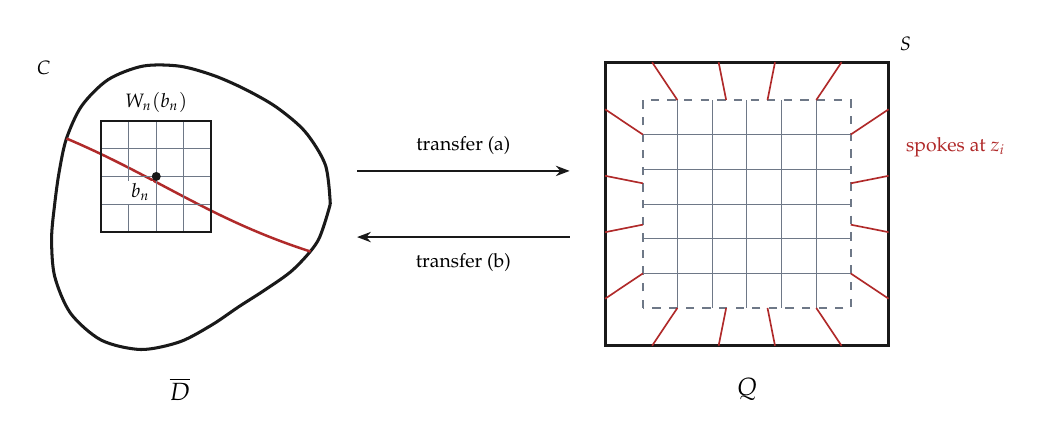
\begin{tikzpicture}[scale=1.0]
  % ---- source side ----
  \begin{scope}[shift={(-3.6,0)}]
    \def\blc{1.75+0.16*cos(3*\t)+0.10*sin(2*\t)}
    \fill[white] plot[domain=0:360,smooth,variable=\t] ({\t}:{\blc});
    \draw[jcurve] plot[domain=0:360,smooth,variable=\t] ({\t}:{\blc});
    \draw[cut,line width=0.9pt] (150:{1.75+0.16*cos(450)+0.10*sin(300)})
       .. controls (-0.3,0.35) and (0.4,-0.2) ..
       (-20:{1.75+0.16*cos(-60)+0.10*sin(-40)});
    \foreach \i in {0,...,4} {
      \draw[aux,line width=0.35pt] (-1.0+0.35*\i,-0.35) -- (-1.0+0.35*\i,1.05);
      \draw[aux,line width=0.35pt] (-1.0,-0.35+0.35*\i) -- (0.4,-0.35+0.35*\i);}
    \draw[curve,line width=0.7pt] (-1.0,-0.35) rectangle (0.4,1.05);
    \node[jdot] at (-0.3,0.35) {};
    \node[font=\scriptsize,fill=white,inner sep=1pt,anchor=north east]
       at (-0.34,0.30) {$b_n$};
    \node[font=\scriptsize,fill=white,inner sep=1pt,anchor=south]
       at (-0.3,1.12) {$W_n(b_n)$};
    \node[font=\scriptsize,anchor=south east] at (135:2.15) {$C$};
    \node[font=\small] at (0,-2.35) {$\overline D$};
  \end{scope}
  % ---- target side ----
  \begin{scope}[shift={(3.6,0)}]
    \draw[jcurve] (-1.8,-1.8) rectangle (1.8,1.8);
    \draw[aux,line width=0.55pt,dashed] (-1.32,-1.32) rectangle (1.32,1.32);
    \foreach \i in {1,...,5} {
      \draw[aux,line width=0.35pt] (-1.32+0.44*\i,-1.32) -- (-1.32+0.44*\i,1.32);
      \draw[aux,line width=0.35pt] (-1.32,-1.32+0.44*\i) -- (1.32,-1.32+0.44*\i);}
    \foreach \k in {0,...,15} {
      \pgfmathsetmacro{\an}{22.5*\k+11.25}
      \draw[cut,line width=0.6pt]
        ({1.8*cos(\an)/max(abs(cos(\an)),abs(sin(\an)))},
         {1.8*sin(\an)/max(abs(cos(\an)),abs(sin(\an)))}) --
        ({1.32*cos(\an)/max(abs(cos(\an)),abs(sin(\an)))},
         {1.32*sin(\an)/max(abs(cos(\an)),abs(sin(\an)))});}
    \node[font=\scriptsize,anchor=south west] at (1.82,1.82) {$S$};
    \node[cut,font=\scriptsize,anchor=west] at (1.9,0.72) {spokes at $z_i$};
    \node[font=\small] at (0,-2.35) {$Q$};
  \end{scope}
  % ---- the two transfers ----
  \draw[curve,line width=0.6pt,-{Stealth[length=5pt]}] (-1.35,0.42) -- (1.35,0.42);
  \draw[curve,line width=0.6pt,-{Stealth[length=5pt]}] (1.35,-0.42) -- (-1.35,-0.42);
  \node[font=\scriptsize,anchor=south] at (0,0.50) {transfer (a)};
  \node[font=\scriptsize,anchor=north] at (0,-0.50) {transfer (b)};
\end{tikzpicture}
\caption{One stage of the scheme. A grid fine enough to force cells
below $\varepsilon_n$ is attached to the source inside the square
$W_n(b_n)$ and carried to the target; then an anchored mesh --- a
gridded core $\lambda Q$ and a collar cut into rectangles by spokes
dropped from fresh anchor points $z_i\in u(\mathcal A)$ --- is laid over the
target and carried back. Refining one side alone would shrink that
side's cells only; the alternation shrinks
both.}\label{fig:stage}
\end{figure}

Stage $n$ starts from $(\Gamma_{n-1},\Gamma_{n-1}')$ and performs four
steps (Figure~\ref{fig:stage}): attach a local grid in $W_n(b_n)$ to the source
(Proposition~\ref{prop:grid}); transfer it to the target
(Theorem~\ref{thm:transfer}(a)); refine the whole target by the
anchored mesh with $\delta=\varepsilon_n$
(Proposition~\ref{prop:mesh}); transfer back
(Theorem~\ref{thm:transfer}(b)). The result is
$(\Gamma_n,\Gamma_n')$.

\begin{proposition}[Local grid]\label{prop:grid}
There is a 2-connected extension $H_n\supseteq\Gamma_{n-1}$, polygonal
off $C$, with $|H_n|\setminus C$ connected, containing a full
rectangular grid on $W=W_n(b_n)$ whose lines belong to the skeleton
and whose closed rectangles have diameter $<\varepsilon_n$.
\end{proposition}
\begin{proof}
Let $K$ be such a grid on $W$ (mesh below $\varepsilon_n/2$),
subdivided against the inner skeleton of $\Gamma_{n-1}$
(Lemma~\ref{lem:graphfacts}(f)). If the two graphs share at least two
vertices, their union is 2-connected
(Lemma~\ref{lem:graphfacts}(c)). If they share none, $K$ lies in one
face $F$ (a bounded Jordan region); take a straight grid edge $J$ with
supporting line $\ell$: the component of $\ell\cap F$ containing
$J^\circ$ is a bounded open segment of $\ell$ whose closure $E$ is a
segment with two distinct endpoints on $\partial F$ and interior in
$F$ --- a crosscut --- and after adding the ear $E$
(Lemma~\ref{lem:graphfacts}(d)) the graphs share two vertices along
$J$. If they share exactly one vertex $x$, the connected set
$K\setminus\{x\}$ lies in one face; run the same line construction
through a grid-edge point $y\ne x$, along a line missing $x$, giving a
crosscut $E$ with $x,y$ as two common points. In each case the union,
overlaid, is 2-connected and contains the grid.

Its inner part may be disconnected (an auxiliary crosscut may
have both ends on $C$). While it is, pick points in two components,
join them by a simple polygonal arc in the region $D$
(Lemma~\ref{lem:polyconn}), and overlay: each component of the arc
outside the graph is an ear; ears preserve 2-connectivity, no ear
creates a new component of the inner part since the arc lies in
$D$, and once all its ears are present the whole arc joins the two
chosen components inside the inner part. Each round strictly
lowers the number of components, so finitely many rounds finish.
\end{proof}

\begin{proposition}[Anchored mesh]\label{prop:mesh}
For every $\delta>0$ there is a polygonal cellulation $T$ of $Q$ whose
faces have diameter $<\delta$, whose skeleton is 2-connected with
$|T|\setminus S$ connected, in which every prescribed boundary vertex
of $\Gamma_{n-1}'$ appears, and whose only new edges meeting $S$ are
single \emph{spokes}, one at each of finitely many fresh points of
$u(\mathcal A)$.
\end{proposition}
\begin{proof}
Radial coordinates $x=tz$ ($t=\|x\|_\infty$, $z\in S$) identify the
collar $Q\setminus(\lambda Q)^\circ$ with $S\times[\lambda,1]$; fix
$\lambda<1$ with $\sqrt2(1-\lambda)<\delta/4$. Parametrize $S$ by a
circle, partition it into arcs of image-diameter $<\delta/8$ (uniform
continuity), and choose one fresh point $z_i$ of the dense set
$u(\mathcal A)$ in the relative interior of each, avoiding the finitely many
excluded points --- possible since a dense set meets every open subarc
even after finitely many deletions. Consecutive $z_i$ then bound arcs
$A_i\subseteq S$ of diameter $<\delta/4$; insert the old boundary
vertices as subdivisions of these arcs. Draw the spokes
$[z_i,\lambda z_i]$ --- disjoint, since two radial segments of the
collar meet only on a common ray --- cutting the collar into the
rectangles $R_i=\{tz:z\in A_i,\ \lambda\le t\le1\}$, each of diameter
at most $2\sqrt2(1-\lambda)+\delta/4<\delta$ by the estimate
$\|tz-sw\|\le\|tz-z\|+\|z-w\|+\|w-sw\|$. Grid the core square
$\lambda Q$ with mesh $<\delta/2$ so that its rectangles have diameter
$<\delta$, and overlay everything. The faces are the grid rectangles
and the collar rectangles; the skeleton is 2-connected by
Lemma~\ref{lem:graphfacts}(c): start from the core grid, subdivided
at all the points $\lambda z_i$, which is 2-connected; each
collar-rectangle boundary $\partial R_i$ is a cycle --- two spokes,
one boundary arc, one core arc --- sharing at least the two vertices
$\lambda z_i,\lambda z_{i+1}$ with the graph built so far, so
adjoining these cycles one after another preserves 2-connectivity,
and their union with the grid is the whole skeleton. And
$|T|\setminus S$ is connected: the core grid and $\partial(\lambda Q)$ form a connected
set in $Q^\circ$, to which each spoke minus its outer endpoint is
attached. Overlaying $T$ with $\Gamma_{n-1}'$ preserves 2-connectivity, since
both graphs contain the outer cycle $S$ and so share at least two
vertices (Lemma~\ref{lem:graphfacts}(c)); if the two inner
parts are disjoint, adding the ears of one joining arc in $Q^\circ$,
as in Proposition~\ref{prop:grid}, connects them. This yields the
required refinement; the only new edges meeting $S$ are the spokes.
\end{proof}

\begin{proposition}[Shrinking stars]\label{prop:shrink}
For every $x\in D$ one has $\diam\St_{\Gamma_n}(x)\to0$, and
$\diam\St_{\Gamma_n'}(\sigma_n'(x))\to0$ holds uniformly in $x$;
here
$\sigma_n(x)$ is the carrier of $x$ and $\sigma_n'(x)$ the
corresponding target cell.
\end{proposition}
\begin{proof}
Uniformity on the target: the stage-$n$ target skeleton contains the
mesh of Proposition~\ref{prop:mesh}, so each of its faces, being
connected and disjoint from the mesh skeleton, lies in one mesh face
and has diameter $<\varepsilon_n$; faces only shrink under later
refinement
(each face lies in the closure of its parent), and all closed faces in
a star share a point, so star diameters are $<2\varepsilon_n$.

On the source, fix $x$ and $d=r(x)>0$; choose $b\in B$ with
$\|b-x\|_\infty<d/8$, occurring at arbitrarily large indices $n$ with
$\varepsilon_n<d/8$. Then $r(b)>7d/8$, so
$s_n(b)\ge r(b)-\varepsilon_n>3d/4>d/8$, and $x$ lies in the interior
of $W_n(b)$. At the stage-$n$ pullback, every face of $\Gamma_n$
incident with $x$ has, by parent compatibility, a parent face $T$ in
the pre-pullback source cellulation with $x\in\overline T$; $T$ is
connected and disjoint from that skeleton, which contains all grid
lines of $W$ and $\partial W$, so $T$ lies in one component of their
complement, and not in the unbounded one, whose closure misses the
interior point $x$; hence $T$ lies in one open grid rectangle and
$\overline T$ in its closure, of diameter $<\varepsilon_n$. All closed
faces of $\St_{\Gamma_n}(x)$ contain $x$, so
$\diam\St_{\Gamma_n}(x)<2\varepsilon_n$; and stars only shrink at
later stages.
\end{proof}

Let $\mathcal A_\infty\subseteq\mathcal A$ be the preimages of all fresh anchors ever
used. Since stage-$n$ anchors cut $S$ into arcs of diameter
$<\varepsilon_n/4$, the set $u(\mathcal A_\infty)$ is dense in $S$; and
$\mathcal A_\infty$ is dense in $C$ because $u^{-1}$ is a continuous surjection.
When an anchor is introduced its spoke is an inner edge at it,
and an initial subedge of the spoke remains incident at all later
stages.

\section{The interior homeomorphism}\label{sec:interior}

Everything is now in place. For $x\in D$ let $T_n(x)$ be the closed
target star of $\sigma_n'(x)$. Parent compatibility makes these nested,
and Proposition~\ref{prop:shrink} drives their diameters to zero, so by
Lemma~\ref{lem:nested} their intersection is a single point. That point
is the image of $x$:
\[
  \{F(x)\}\;:=\;\bigcap_{n\ge1}T_n(x).
\]
Write $G_n=|\Gamma_n|$ and $G_n'=|\Gamma_n'|$; the skeleton
homeomorphisms $g_n$ are nested and combine to a bijection
$g_\infty:\bigcup_nG_n\to\bigcup_nG_n'$.

\begin{proposition}[The interior map]\label{prop:homeo}
$F:D\to Q^\circ$ is a homeomorphism, and $F=g_n$ on
$G_n\cap D$ for every $n$.
\end{proposition}
\begin{proof}
Throughout, we use: for any point $y$ of a closed domain, the
complement of the union of the closed cells not containing $y$ is a
relative neighborhood $U$ of $y$ in which every carrier is a supercell
of the carrier of $y$ (a carrier whose closure missed $y$ would be
excluded; then the frontier property applies). Call this the
\emph{star neighborhood} at $y$.

\emph{Agreement.} For $x\in G_N\cap D$ and $n\ge N$, the skeleton map
carries the carrier of $x$ onto the corresponding cell, so
$g_N(x)=g_n(x)\in T_n(x)$; hence $F(x)=g_N(x)$.

\emph{Continuity.} Given $x$ and $\eta$, pick $n$ with
$\diam T_n(x)<\eta$; in the stage-$n$ source star neighborhood at $x$,
shrunk into $D$, every point $z$ has carrier above that of $x$, the
corresponding target relation holds (Lemma~\ref{lem:corr}), so
$T_n(z)\subseteq T_n(x)$ and $\|F(z)-F(x)\|<\eta$.

\emph{Interior image.} Choose $n$ with the source star of $x$ smaller
than $\dist(x,C)$, hence disjoint from $C$; the corresponding target
star misses $S$ (Lemma~\ref{lem:corr}), so $F(x)\in Q^\circ$.

\emph{Injectivity.} If $F(x)=F(y)$, the target stars of $x,y$ meet at
every stage, hence so do the source stars
(Lemma~\ref{lem:corr}); a common point gives
$\|x-y\|\le\diam\St_{\Gamma_n}(x)+\diam\St_{\Gamma_n}(y)\to0$.

\emph{Surjectivity.} Skeleton points off $S$ are dense in $Q^\circ$:
every face has small diameter and its boundary contains an inner
edge. Given $y\in Q^\circ$, take skeleton points $y_k\to y$ off $S$
and $x_k=g_\infty^{-1}(y_k)\in D$. Choose $n$ with the target star of
$y$ off $S$, and its target star neighborhood $V$; let $K$ be the
union of the source closed cells corresponding to the finitely many
supercells of the carrier of $y$: by Lemma~\ref{lem:corr}, $K$ is a
compact subset of $D$. For large $k$, $y_k\in V$, and viewing
$x_k,y_k$ as corresponding skeleton points at a late common stage,
their stage-$n$ carriers correspond; so $x_k\in K$. The sequence
$x_k$ has a limit point $x\in K\subseteq D$ along a subsequence, and
by continuity and agreement $F(x)=\lim y_k=y$.

\emph{Cells map to cells.} For corresponding inner open cells:
on vertices and edges $F=g_n$. For a face $R$: by
Lemma~\ref{lem:cellgeom}(d) the closed star of $R$ is $\overline R$
itself, so $F(R)\subseteq\overline{R'}$, and indeed
$F(R)\subseteq R'$: a value on $\partial R'$, which lies in the
target skeleton and in $Q^\circ$, has a source-skeleton preimage in
$D$ at which $F$ agrees with $g_n$, contradicting injectivity. For
the converse, a preimage in $D$ of a point of $R'$ cannot have a
vertex or edge carrier (its image would be a skeleton point), so its
carrier is a face $R_0$ with $F(R_0)\subseteq R_0'$ meeting $R'$;
faces are disjoint, so $R_0=R$. Thus $F(R)=R'$.

\emph{Inverse continuity.} Given $y=F(x)$ and $\eta$, pick $n$ with
the source star of $x$ smaller than $\eta$ and take the target star
neighborhood $V$ at $y$: for $z\in V\cap Q^\circ$, the target carrier
of $y$ is below that of $z$; transferring and applying the previous
paragraph, the source carrier of $x$ is below that of $F^{-1}(z)$, so
$F^{-1}(z)$ lies in the source star of $x$ and
$\|F^{-1}(z)-x\|<\eta$.
\end{proof}

\section{Continuity at the Jordan curve, and the square extension}\label{sec:boundary}

Extend $F$ to $\overline F:\overline D\to Q$ by $\overline F=u$ on
$C$; it is a bijection onto $Q$, continuous on $D$, and we must prove
continuity at each $p\in C$.

\begin{lemma}[Skeleton crosscuts]\label{lem:skelcross}
For distinct $a,b\in \mathcal A_\infty$ in a common finite stage, there is a
crosscut $P$ of $D$ from $a$ to $b$ inside the stage's skeleton, whose
image $P'=g(P)$ is a crosscut of $Q^\circ$ from $u(a)$ to $u(b)$.
\end{lemma}
\begin{proof}
Write $X=|\Gamma|\setminus C$, a connected set. If some inner
edge has both endpoints on $C$, its interior is clopen in $X$, hence
all of $X$, and $a,b$, being incident with inner edges
(anchors), are its endpoints: take that edge. Otherwise let $\Lambda$
be the vertices and edges entirely in $D$; attaching to each of its
components the half-open interiors of edges with one endpoint on $C$
partitions $X$ into clopen pieces, one per component, so $\Lambda$ is
connected (and nonempty, via the edge at $a$). The union of $\Lambda$
with the two edges at $a,b$ is then connected and meets $C$ exactly in
$\{a,b\}$; a simple graph path from $a$ to $b$ inside it is the
crosscut. Its image under the skeleton homeomorphism is simple, meets
$S$ exactly at $u(a),u(b)$, and is polygonal in $Q^\circ$.
\end{proof}

\begin{lemma}[Sides correspond]\label{lem:sides}
With $P,P'$ as above, label the components of $D\setminus P$ by
$\overline{U_i}\cap C=A_i$ and of $Q^\circ\setminus P'$ by
$\overline{U_i'}\cap S=u(A_i)$ \textup(Theorem~\ref{thm:cross}\textup).
Then $F(U_i)=U_i'$.
\end{lemma}
\begin{proof}
$F$ is a homeomorphism agreeing with $g$ on $P\cap D$, so it maps the
components of $D\setminus P$ onto those of $Q^\circ\setminus P'$; only
the labels need identifying. Pick $c\in \mathcal A_\infty$ in the relative
interior of $A_i$, at a stage containing $P$, $c$, and an inner
edge $e$ at $c$. Since $\overline{U_{3-i}}\cap C=A_{3-i}$ misses $c$,
a short initial subarc $J$ of $e$, with $c$ removed, avoids
$\overline{U_{3-i}}$ and $P$, hence lies in $U_i$; likewise its image
$g(J)$, short enough, lies in $U_i'$. As $F(J)=g(J)$, the labels
match.
\end{proof}

\begin{proposition}[Boundary continuity]\label{prop:bdry}
$\overline F$ is continuous, hence a homeomorphism
$\overline D\to Q$; this proves Theorem~\ref{thm:square}.
\end{proposition}
\begin{proof}
Suppose $x_k\to p\in C$ in $D$ but
$\overline F(x_k)\not\to u(p)$. Passing to a subsequence in the
compact set $Q$, $F(x_k)\to q\ne u(p)$; and $q\in S$, since a limit in
$Q^\circ$ would force $x_k\to F^{-1}(q)\in D$. Let $r=u^{-1}(q)\ne p$.
By density of $\mathcal A_\infty$, choose $a,b\in \mathcal A_\infty$, distinct from
$p,r$, separating them on $C$; the stages being nested, $a,b$ share a
finite stage, giving crosscuts $P,P'$
(Lemma~\ref{lem:skelcross}). Let $U_1,U_2$ be the two sides of $P$,
labelled so that $\overline{U_i}\cap C=A_i$ with $p$ interior to $A_1$.
Two compact sets are to be avoided near $p$: the crosscut $P$ itself,
which misses $p$ because $P\cap C=\{a,b\}$, and $\overline{U_2}$, which
misses $p$ because $\overline{U_2}\cap C=A_2$
(Theorem~\ref{thm:cross}). So some neighborhood of $p$ meets neither,
and every $x_k$ near $p$ lies in $U_1$ --- not merely in its closure.
By Lemma~\ref{lem:sides} the images lie in $U_1'$, so
$q=\lim\overline F(x_k)$ lies in $\overline{U_1'}$, whose intersection
with $S$ is $u(A_1)$. But $q=u(r)$ with $r$ interior to $A_2$ ---
contradiction. Continuity of the bijection $\overline F$ on the
compact set $\overline D$ makes it a homeomorphism onto $Q$. For
sequences approaching $p$ within $C$, continuity is that of $u$;
mixed sequences follow by combining. \end{proof}

\section{From the square extension to the plane}\label{sec:plane}

Only the exterior is left. Inversion in a point of $\Int(C)$ turns the
closed exterior into a closed interior punctured at one point, so the
theorem just proved applies to it --- provided the two extensions can be
made to agree at that point, which is what the pointed version below
arranges.

\begin{lemma}[Moving a point of the square]\label{lem:mover}
For interior points $x,y$ of $Q$ there is a homeomorphism of $Q$
fixing $S$ pointwise and sending $x$ to $y$.
\end{lemma}
\begin{proof}
The four triangles on $x$ and the sides of $Q$ triangulate $Q$; map
each affinely to the triangle on $y$ and the same side, fixing the two
side vertices and sending $x\to y$. Adjacent maps agree on shared
segments (affine maps agreeing at two points agree on their line), and
each fixes its side of $S$ pointwise; paste, and construct the inverse
the same way with the roles of $x,y$ reversed.
\end{proof}

\begin{proposition}[Pointed extension]\label{prop:pointed}
Given $f:C\to C'$ and interior points $z\in\Int(C)$,
$z'\in\Int(C')$, some extension of $f$ to the closed interiors sends
$z$ to $z'$.
\end{proposition}
\begin{proof}
Choose a homeomorphism $C'\to S$ (Lemma~\ref{lem:circle}) and extend
it to $\Theta:C'\cup\Int(C')\to Q$ (Theorem~\ref{thm:square}); let
$\Phi$ be an extension of $f$ from Proposition~\ref{prop:reduce}.
Insert the mover $M$ (Lemma~\ref{lem:mover}) carrying $\Theta(\Phi(z))$
to $\Theta(z')$: then $\Theta^{-1}\circ M\circ\Theta\circ\Phi$ extends
$f$ and sends $z\mapsto z'$.
\end{proof}

\begin{lemma}[Inversion]\label{lem:inversion}
For $a\in\Int(C)$, the inversion $I_a(x)=a+(x-a)/\|x-a\|^2$ maps
$C$ onto a Jordan curve $C^a$ and restricts to a homeomorphism of
$C\cup\Ext(C)$ onto $\bigl(C^a\cup\Int(C^a)\bigr)\setminus\{a\}$.
\end{lemma}
\begin{proof}
$I_a$ is an involutive homeomorphism of $\mathbb R^2\setminus\{a\}$,
so $C^a=I_a(C)$ is a Jordan curve. Let
$U=I_a(\Ext(C))\cup\{a\}$: open away from $a$, and open at $a$
because the complement of a large disk maps into a punctured small
disk at $a$; connected, since $a$ lies in the closure of the connected
image; and bounded, since $\Ext(C)$ avoids the ball
$B(a,\dist(a,C))\subseteq\Int(C)$. Away from $a$, boundaries
correspond under the homeomorphism, so $\partial U=C^a$
(with $a$ interior to $U$). Then $U$ is clopen in the component of
$\mathbb R^2\setminus C^a$ containing it, hence equals it; being
bounded, that component is $\Int(C^a)$
(Theorem~\ref{thm:jct}). Removing $a$ and adding $C\to C^a$ gives the
stated restriction.
\end{proof}

\begin{proof}[Proof of Theorem~\ref{thm:main}]
Extend $f$ over the closed interiors to
$F_{\mathrm{int}}:C\cup\Int(C)\to C'\cup\Int(C')$
(Proposition~\ref{prop:reduce}). For the exteriors, pick
$a\in\Int(C)$, $b\in\Int(C')$ and set
$f^*=I_b\circ f\circ I_a:C^a\to(C')^b$. By
Proposition~\ref{prop:pointed} extend $f^*$ to
$\Phi^*$ over the closed interiors with $\Phi^*(a)=b$; then
\[
F_{\mathrm{ext}}
 =I_b\circ \Phi^*\circ I_a
 :\;C\cup\Ext(C)\longrightarrow C'\cup\Ext(C'),
\]
using Lemma~\ref{lem:inversion} on both sides and removing the
corresponding points $a,b$, is a homeomorphism extending
$I_b\circ f^*\circ I_a=f$ on $C$. The maps
$F_{\mathrm{int}},F_{\mathrm{ext}}$ agree on $C$ and are defined on
the two closed sets $C\cup\Int(C)$ and $C\cup\Ext(C)$ covering the
plane; pasting them, and pasting their inverses on
$C'\cup\Int(C')$ and $C'\cup\Ext(C')$, yields the desired
homeomorphism of $\mathbb R^2$ extending $f$.
\end{proof}

\section*{What the proof used}

It is worth recording how little went in. Beyond the metric topology of
the plane --- compactness, connectedness, uniform continuity --- and the
density of $\mathbb Q^2$, the argument rests on one counting function,
three constructions, and a single nonplanarity fact.

The counting function is the crossing parity $\pi_C$ of
Section~\ref{sec:polygonal}. It is what makes the polygonal count exact:
the strip lemma bounds the number of components by two, and $\pi_C$,
taking both values, shows the bound is attained. The identity
$\pi_C=\pi_{J_1}+\pi_{J_2}$ is then the entire content of the polygonal
crosscut theorem.

The three constructions are the two-sided strip, which manufactures the
sides of a polygonal curve; the chain of squares, which buries a simple
arc so thoroughly that its complement never notices it; and the matched
cellulation, which replaces the homeomorphism being sought by a sequence
of finite ones and lets a limit do the rest.

The nonplanarity fact is that $K_{3,3}$ has no plane drawing. It is
invoked exactly twice, and both times to forbid a curve from separating
wrongly: once against a curve that separates too little --- not at all
--- and once against one that separates too much, into three regions.
Between those two applications lies the whole distance from polygons to
arbitrary Jordan curves.

\section*{Note}
The detailed companion manuscript proves the same theorem along the
same route with every inference expanded to formalization granularity,
together with a mechanically generated citation index and an explicit
imported-background appendix. Where the present text says ``by the
correspondence of incidences'' or compresses a constructor case check
into a sentence, the companion contains the full case analysis.

\end{document}
